\documentclass[12pt,letterpaper]{article}

% Essential packages
\usepackage[utf8]{inputenc}
\usepackage[T1]{fontenc}
\usepackage[english]{babel}
\usepackage{amsmath,amsfonts,amssymb}
\usepackage{graphicx}
\usepackage[table,xcdraw]{xcolor}
\usepackage{booktabs}
\usepackage{array}
\usepackage{multirow}
\usepackage{multicol}

% Page layout and formatting
\usepackage[margin=1in]{geometry}
\usepackage{setspace}
\usepackage{fancyhdr}
\usepackage{titlesec}
\usepackage{caption}
\usepackage{subcaption}

% References and citations
\usepackage[style=numeric,backend=bibtex,sorting=none]{biblatex}
\addbibresource{references.bib} % Create this file for your references

% Table of contents formatting
\usepackage{tocloft}
\usepackage{hyperref}
\hypersetup{
    colorlinks=true,
    linkcolor=black,
    filecolor=magenta,      
    urlcolor=blue,
    citecolor=blue
}

% Figure and table numbering
\usepackage{chngcntr}
\counterwithin{figure}{section}
\counterwithin{table}{section}

% Figure Filepath
\graphicspath{{/home/msmitty/Documents/TransientBloodRheo_summerExperience/WritingMaterials/0.Figures/}}

% Custom formatting for captions
\captionsetup{
    font=small,
    labelfont=bf,
    format=plain,
    justification=centering,
    margin=0.5cm
}

% Header and footer
\pagestyle{fancy}
\fancyhf{}
\rhead{\thepage}
\lhead{DRAFT--Transient Blood Rheology--DRAFT}
\renewcommand{\headrulewidth}{0.4pt}

% Title formatting
\titleformat{\section}{\large\bfseries}{\thesection}{1em}{}
\titleformat{\subsection}{\normalsize\bfseries}{\thesubsection}{1em}{}
\titleformat{\subsubsection}{\normalsize\itshape}{\thesubsubsection}{1em}{}

% Line spacing
\onehalfspacing

\begin{document}

% Title page
\begin{titlepage}
    \centering
    \vspace*{2cm}
    
    {\LARGE\bfseries DRAFT -- Main Title Here -- DRAFT\par}
    
    \vspace{1.5cm}
    
    {\large A Machine Learning Approach to Correlating Physiological Parameters with Rheological Features\par}
    
    \vspace{2cm}
    
    {\Large A Manning Smith\par}
    \vspace{0.5cm}
    {\large University of Delaware\par}
    {\large Bioinformatics and Computation Science\par}
    
    \vspace{2cm}
    
    {\large \today\par}
    
    \vfill
    
    \begin{abstract}
    \noindent
    Abstract goes here
    \end{abstract}
    
\end{titlepage}

% Table of contents
\newpage
\tableofcontents

% Introduction
\newpage
\section{Introduction}
Intro section here.

% Methods
\newpage
\section{Methods}
The data sampling methods.. Need from Sean....

This work was all performed using Python version 3.12.3. The utilized packages are outlined in the supplied requirements.txt found in the supplemental resources' section
for reproducibility. Various machine learning methods were utilized in alignment with a dataset comprised of a small sample size. The Scikit-learn package, version 1.6.1
was accessed for all the machine learning techniques. The accuracy of the models was validated through K-Fold Cross Validation. The utilized methods were produced with a
constant random seed of 1743, the year University of Delaware was founded.

To start with data processing it was important to address missing values in the rheological dataset due to the already limited sample size. K-nearest neighbors (KNN)
imputation was used for data imputation to fill out the missing values forming a complete set of rheological data. The KNN algorithm identifies the $k$ most similar
complete observations based on Euclidean distance across all available features, then imputes missing values using the weighted average of these neighbors' corresponding values.
The chosen value of $k=3$ captures local data structure while maintaining robustness against outliers. This approach is well-suited for rheological data, where the parameters often
exhibit strong intercorrelations due to their shared dependence.

Secondly, the physiological variables were standardized using sklearn's StandardScaler, which transforms each feature to have zero mean and unit variance according to:
$$
    z_{ij} = \frac{x_{ij}-\mu_j}{\sigma_j}
$$
where $x_{ij}$ represents the original value for sample $i$ and feature $j$, $\mu_j$ is the sample mean, and $\sigma_j$ is the sample standard deviation for feature $j$.

Standardization was essential for the PCA, as PCA is sensitive to the relative scales of input variables. Without standardization,
variables with larger natural scales (e.g., cholesterol levels in mg/dL) would dominate the principal components over variables with smaller scales (e.g., hematocrit percentages),
leading to biased dimensionality reduction that reflects measurement units rather than biological relationships.

Previous research (cite paper) highlighted viability in the physiological variables, however further dimensional reduction may prove further viability preserving the maximum variance.
PCA transforms the original feature space into a new coordinate system where the axes (principal components) are linear combinations of the original variables,
ordered by the amount of variance they explain.

The mathematical foundation involves eigendecomposition of the covariance matrix:
$$
    C = \frac{1}{n-1} \mathbf{X}^T\mathbf{X}
$$
where $\mathbf{X}$ is the standardized data matrix. The principal components are the eigenvectors of $\mathbf{C}$, and the explained variance for each component corresponds to
its eigenvalue. For the purposes of this research the following 13 features were selected outlined in table XX.

\begin{table}[]
    \centering
    \caption{Physiological targets used for the transient rheology parameterization.}
    \begin{tabular}{lcc}
        Physiology                                & Code & Units \\
        \hline
        Hematocrit                                & HCT  & $\%$ \\
        Fibrinogen                                & FIB  & $mg/dL$ \\
        Total Cholesterol                         & CHOL & $mg/dL$ \\
        Triglycerides                             & TRIG & $mg/dL$ \\
        HDL Cholesterol                           & HDL  & $mg/dL$ \\
        LDL Cholesterol                           & LDL  & $mg/dL$ \\
        White Blood Cell Count                    & WBC  & $\text{thousand}/\mu L$ \\
        Red Blood Cell Count                      & RBC  & $\text{million}/\mu L$ \\
        Hemoglobin                                & HEM  & $g/dL$ \\
        Mean Corpuscular Volume                   & MCV  & $fL$ \\
        Mean Corpuscular Hemoglobin               & MCH  & $pg/cell$ \\
        Mean Corpuscular Hemoglobin Concentration & MCHC & $g/dL$
    \end{tabular}
    \label{need label}
\end{table}

The analysis focused primarily on the first 3 components, which captured the majority of physiological variation while maintaining sufficient sample-to-feature ratios for
robust statistical analysis. Principal component loadings were examined to identify which physiological variables contributed most strongly to each component, enabling biological
interpretation of the reduced feature space.

In starting with the predictability of the PCs Pearson product-moment correlation coefficients were calculated to assess linear relationships between principal components and
rheological parameters. Pearson correlation was selected as the method for showing viability before advancing to further machine learning techniques. Both principal components
and rheological measurements represent continuous variables measured on interval scales, satisfying the data type requirements for parametric correlation analysis.
Principal components are linear combinations of the original physiological variables, making linear correlation analysis theoretically appropriate for detecting associations
with rheological behavior.

Upon showing viability through Pearson correlation, Gaussian Process Regression was implemented to model the complex relationships between PCs derived from physiological
parameters and individual rheological parameters. GPR was selected specifically for its ability to provide uncertainty quantification, handle non-linear relationships,
and perform reasonably well with small datasets. The GPR framework assumes that the target function $f(x)$ follows a Gaussian process defined by $f(x) \approx GP(m(x), k(x,x^{\prime}))$,
where $m(x)$ represents the mean function (set to zero) and $k(x,x^{\prime})$ represents the covariance function that determines similarity between inputs.

The kernel selection strategy employed a composite kernel combining Radial Basis Function and White Noise components according to $k(x,x^\prime)=k_{RBF}(x,x^\prime)+k_{white}(x,x^\prime)$,
where bounded constraints on kernel parameters prevented pathological solutions such as memorization of training points or reduction to pure noise models. The RBF kernel captures smooth,
non-linear relationships through the mathematical formulation $k_{RBF}(x,x^{\prime}) = \sigma^2_f \exp\Big(\frac{-|x-x^{\prime}|^2}{2l^2}\Big)$, where $\sigma^2_f $
represents the signal variance controlling the overall amplitude of function variations, $l$ denotes the length scale parameter determining how quickly correlations decay with
distance between inputs, and $|x-x^{\prime}|^2$ represents the squared Euclidean distance between data points in the principal component space. Hyperparameter bounds set to
length\_scale\_bounds= $(1\times e^{-2}, 1\times e^2)$ and noise\_level\_bounds= $(1\times e^{-5}, 1\times e^0)$ to prevent degenerate solutions while maintaining sufficient
flexibility to capture meaningful physiological-rheological relationships.

For validating the implemented GPR method, K-fold Cross-Validation was utilized. $k=5$ folds was selected to balance the need for adequate training data with robust
performance assessment given the limited sample size of $n=22$. This methodology partitions the dataset into five approximately equal segments, with each segment serving
as a validation set once while the remaining segments form the training set, repeating this process five times with performance metrics calculated for each iteration.
The approach was configured with $n_splits=5$ creating folds containing 4-5 samples each for testing, shuffle=True to randomize sample assignment and prevent systematic
bias from potential temporal ordering in data collection or donor recruitment patterns, and our $random_state=1743$ to ensure reproducible fold assignments across analysis runs.

K-fold cross-validation helped in for identifying various challenges associated with applying GPR to high-dimensional data with small sample sizes.
The cross-validation framework illuminated the severity of overfitting issues inherent in GPR applications to datasets where the sample-to-feature ratio approaches problematic thresholds,
as evidenced by the substantial gap between training performance and validation performance across all folds. This diagnostic capability proved instrumental in understanding the
limitations of the modeling approach and informed subsequent methodological decisions regarding regularization strategies, with the consistent negative performance across folds
providing clear evidence that the challenges were not attributable to specific data partitions or outlier influences but rather represented fundamental mismatches between model
complexity and available training data. The stable, reproducible results obtained through the k-fold framework thus served both to rigorously evaluate model performance and to provide
critical insights into the broader challenges of machine learning applications in small-sample biological datasets.

Given the limitations imposed by the small sample size relative to the high-dimensional feature space, synthetic data generation was employed as a strategy
to augment the training dataset and improve machine learning model performance. Two complementary approaches were implemented to generate realistic synthetic
samples while preserving the underlying statistical relationships in the original dataset.

The fundamental challenge in synthetic data generation for biological systems lies in maintaining both the marginal distributions of individual variables
and the complex correlation structure between physiological and rheological parameters. Simple parametric approaches often fail to capture the non-linear dependencies
present in biological data, while purely random sampling may generate physiologically implausible combinations of values.

The first approach implemented a KNN synthetic data generator that leverages local similarity structures within the original dataset,
operating on the principle that realistic synthetic samples should lie within the convex hull defined by existing observations, particularly near regions of high data density where
the likelihood of encountering similar physiological profiles in real populations is highest. The KNN synthetic generation algorithm proceeds through a systematic four-step process
beginning with seed point selection, where for each synthetic sample a seed point is randomly selected from the original dataset to serve as the basis for generation, ensuring that
all synthetic samples are anchored to actual observed physiological profiles. Neighborhood identification follows, where the $k=3$ nearest neighbors to the seed point are identified
using Euclidean distance in the standardized feature space, with our chosen k to balance between capturing local data structure while maintaining sufficient diversity to
prevent over-reliance on any single neighboring observation.

The second approach employed a Gaussian copula methodology to capture and reproduce the full joint distribution of physiological and rheological variables.
Copula-based methods separate the modeling of marginal distributions from the dependence structure, allowing for flexible representation of complex multivariate relationships.

Variable transformation: Variables are transformed to uniform marginals using rank-based empirical cumulative distribution functions:
$$
    U_{ij} = (rank(X_{ij})+1)/(n+1)
$$
$n$ is the sample size.

New samples are drawn from the multivariate normal distribution and inverse-transformed back to their original scales.
For enhancing the relationships between the variables KNN imputation methods were used to preserve the original data structure utilizing information from similar cases.

Model performance was evaluated using multiple complementary metrics to provide a comprehensive assessment of predictive capability.
The Cross-Validated $R^2$ Score served as the primary performance metric. The $R^2_{CV}$ represents the proportion of variance explained in the response variable.
This metric provides an unbiased estimate of the models explanatory power. Values closer to 1 suggest better predictive performance. The $R^2_{train}$ was calculated on the
training dataset used in fitting the model. This metric helps as a baseline when comparing the cross-validation. Other metrics such as Mean Squared Error Cross-Validation ($MSE_{CV}$)
quantifying the prediction error magnitude, helping to show predictive accuracy on the unseen data. Then the overfitting assessment serves as an evaluation of assessing the models'
generalization capability, calculated as the combination of the and $R^2_{CV}$ and $MSE_{CV}$.

While formal multiple comparison corrections were not applied due to the exploratory nature of the analysis,
results were interpreted with appropriate caution. The focus was placed on identifying patterns and effect sizes rather than definitive statistical conclusions,
with emphasis on replication and validation in future larger datasets. The hierarchical nature of the analysis (PCA followed by correlation analysis) was considered when
interpreting statistical significance, recognizing that the reduced feature space may concentrate signal while also potentially introducing bias in significance testing.
This methodological framework provides a comprehensive approach to analyzing the relationship between physiological blood parameters and rheological behavior while acknowledging
and addressing the inherent challenges of working with limited sample sizes in complex biological systems.

% Results and Discussion
\newpage
\section{Results}
Analysis of the 22-donor dataset revealed distinct patterns in the relationships between physiological blood parameters and rheological constitutive model parameters,
with machine learning approaches successfully identifying key physiological predictors for several rheological variables.

To address the missing values in the rheological dataset, KNN imputation was employed, resulting in a complete dataset with no missing values. There were
5 observations with missing values in the rheological dataset, which were imputed. These missing values were non-random but due to data collection issues.
The transient measure with missing values are seen in (Table \ref{tab:transientRheo}).

\begin{table}[ht]
    \centering
    \caption{Physiological targets used for the transient rheology parameterization.}
    \begin{tabular}{lcc}
        Transient Description                              & Parameter & Units \\
        \hline
        Overall reouleaux rebuild time constant            & $\tau_{\lambda}$  & $s$ \\
        Rouleaux elastic modulus                           & $G_R$  & Pa \\
        RBCs elastic modulus                               & $G_C$ & Pa
    \end{tabular}
    \label{tab:transientRheo}
\end{table}

The imputation process preserved the overall distribution of the rheological parameters while filling in gaps, allowing for subsequent analysis without introducing
significant bias. The imputed distribution of $\tau_{\lambda}$ and $G_R$, decreased the mean and standard deviation slightly (Figure \ref{fig:s1001}). With imputed distribution of $G_C$ the mean
and standard deviation decreased as well, but added much more right skew to the distribution with multiple outliers in the top $25\%$ of the data (Figure \ref{fig:s1002}).

\begin{figure}[ht]
    \centering
    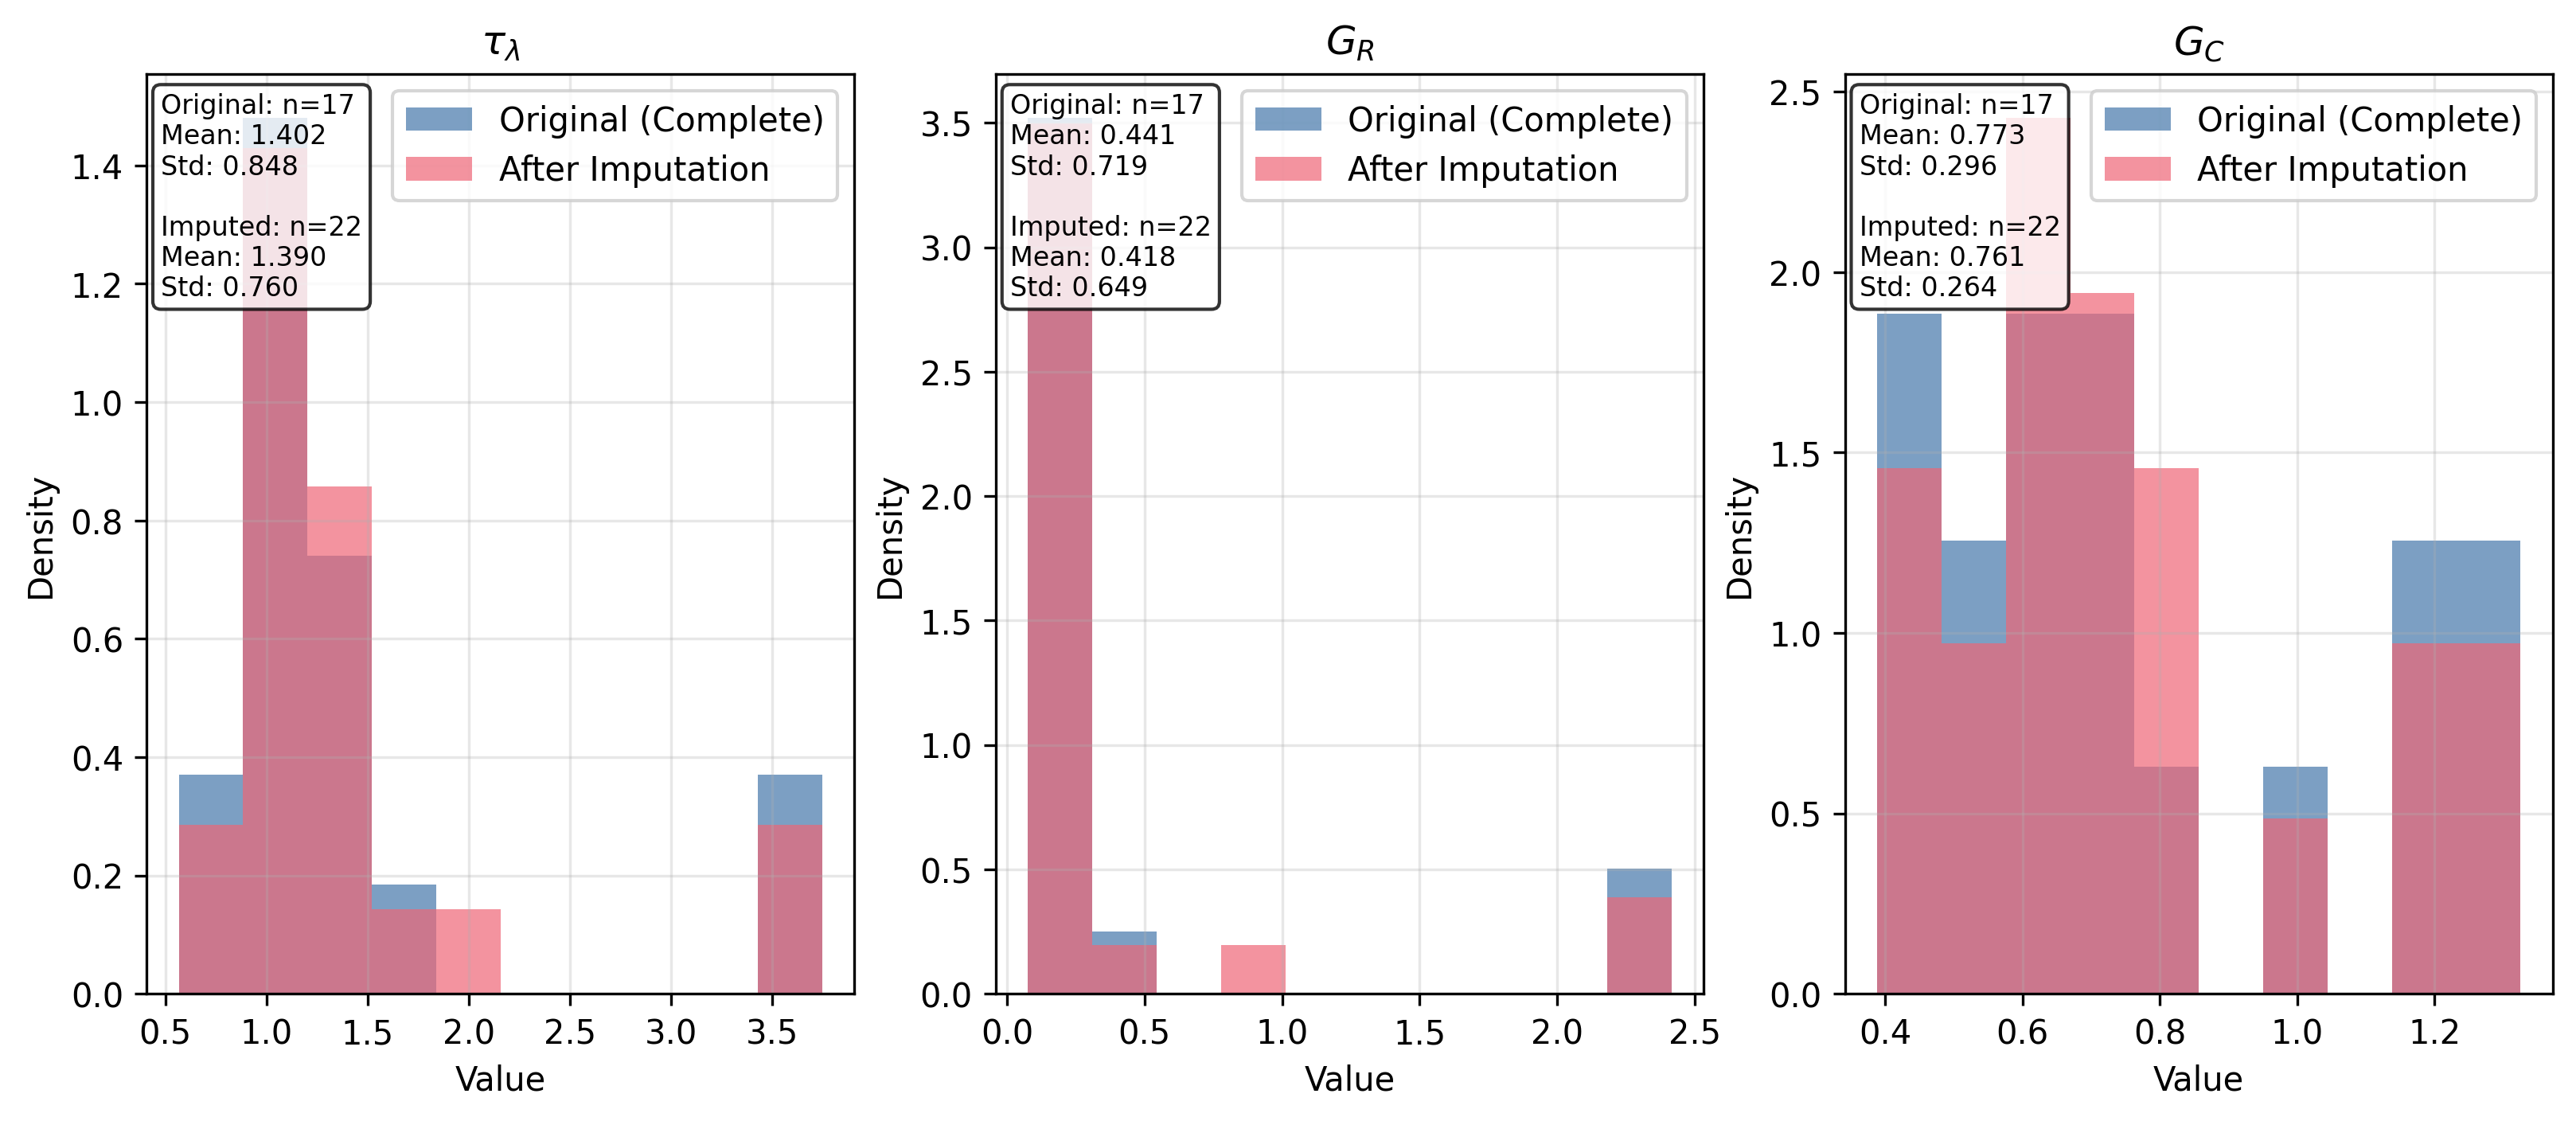
\includegraphics[width=\textwidth]{/home/msmitty/Documents/TransientBloodRheo_summerExperience/WritingMaterials/0.Figures/s1_001_distributions.png}
    \caption{ADD CAPTION}
    \label{fig:s1001}
\end{figure}

\begin{figure}[ht]
    \centering
    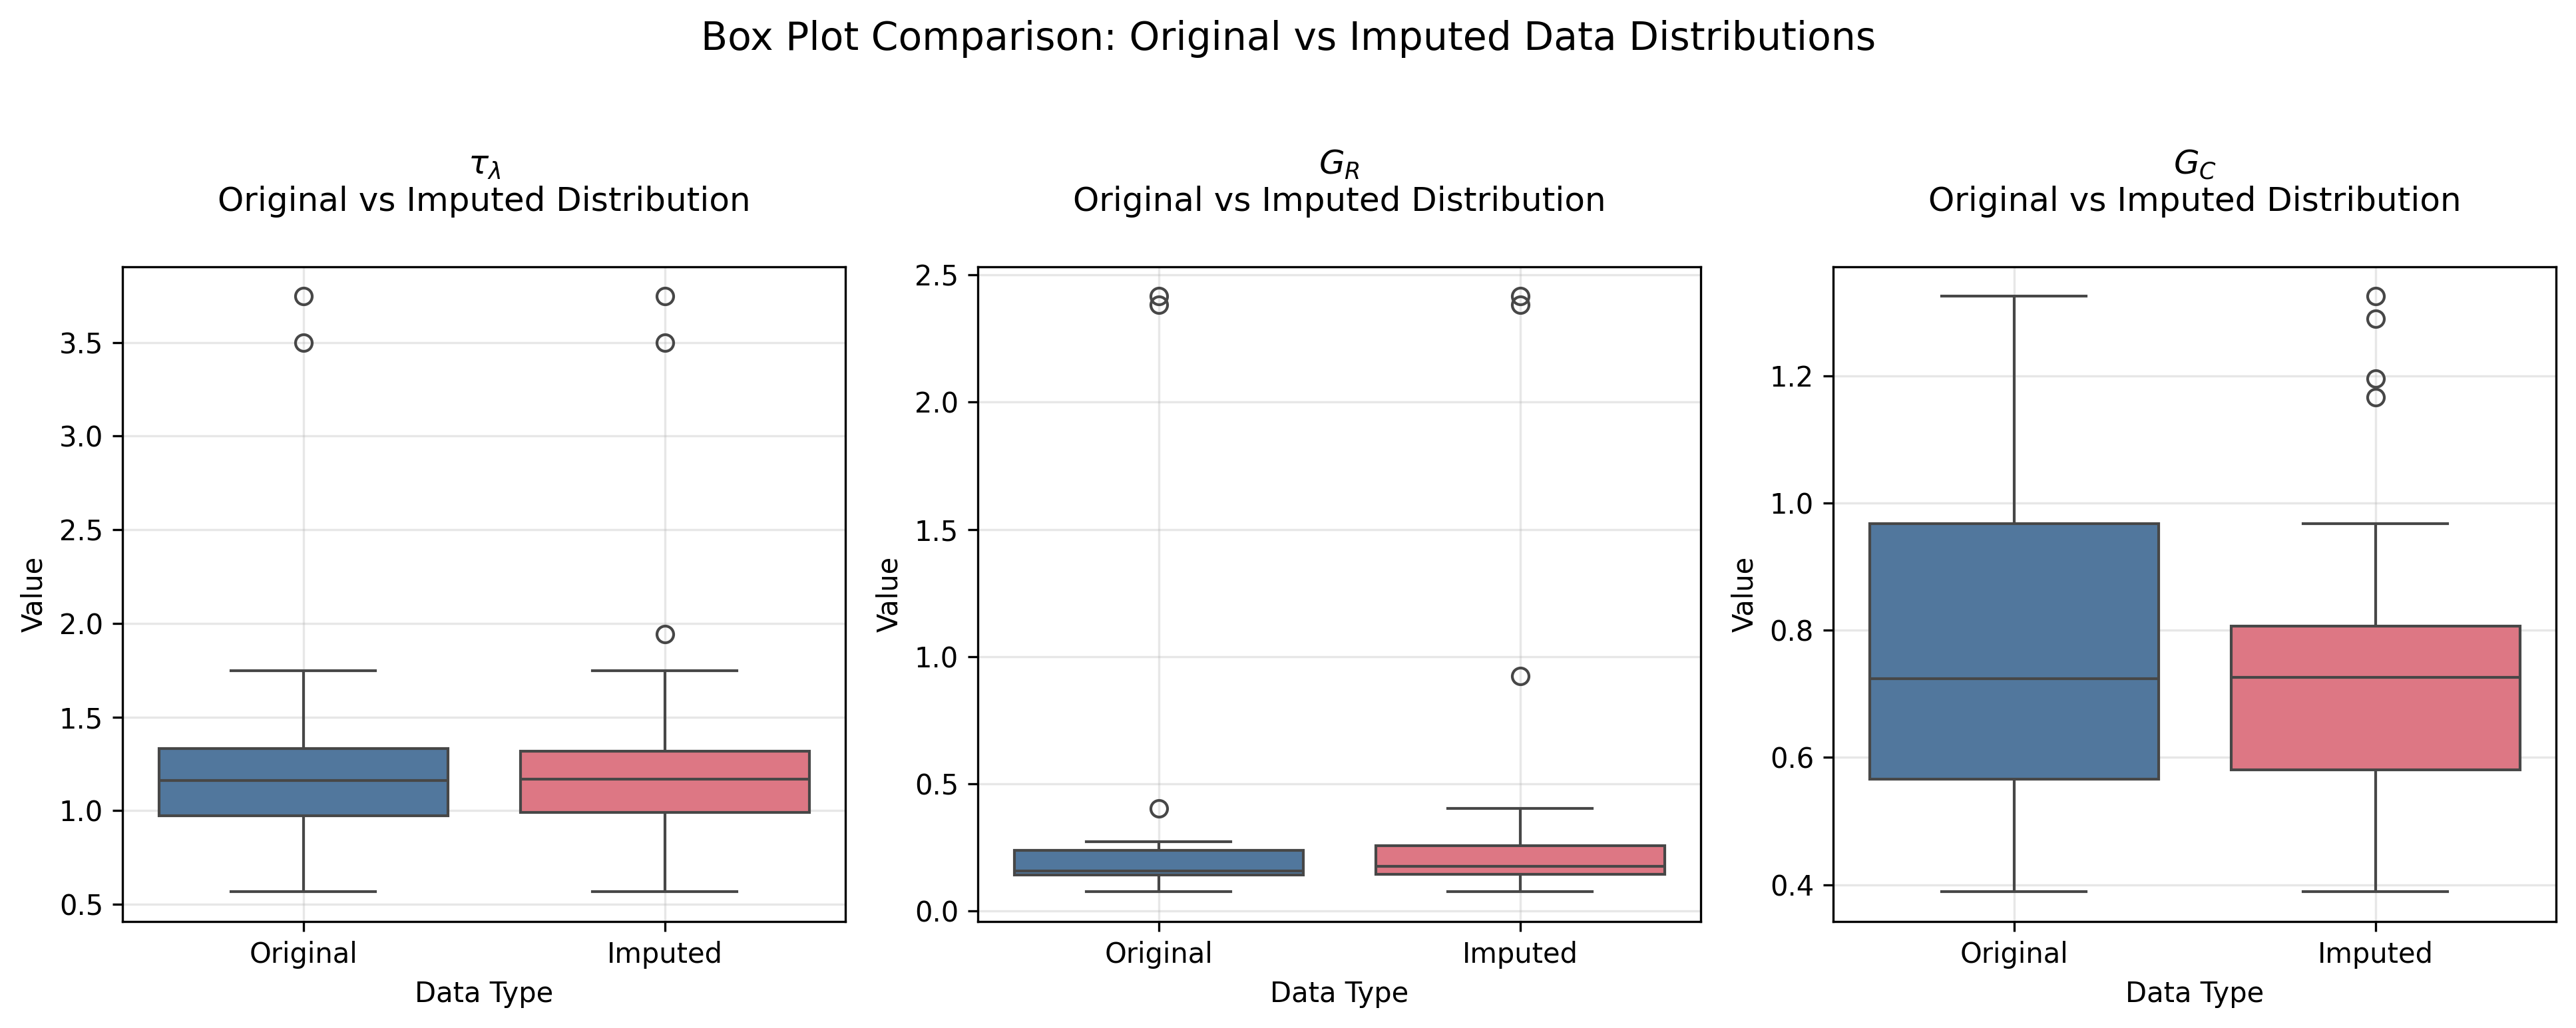
\includegraphics[width=\textwidth]{/home/msmitty/Documents/TransientBloodRheo_summerExperience/WritingMaterials/0.Figures/s1_002_boxplotComparison.png}
    \caption{ADD CAPTION}
    \label{fig:s1002}
\end{figure}

NEED TRANSITION

The first two components explained $\approx 52\%$ of the variance in the data, with PC1 explaining $\approx 31\%$ and PC2 explaining $~21\%$ (Figure \ref{fig:s2004}).
The first three components explained $\approx 67\%$ of the variance in the data, with PC3 explaining $\approx 15\%$ of the variance (Figure \ref{fig:s2003}). The first three components
were selected for further analysis as they captured the majority of physiological variation while maintaining sufficient sample-to-feature ratios for robust statistical analysis.
Principal component loadings were examined to identify which physiological variables contributed most strongly to each component, enabling biological interpretation of the reduced feature space.
\begin{figure}[ht]
    \centering
    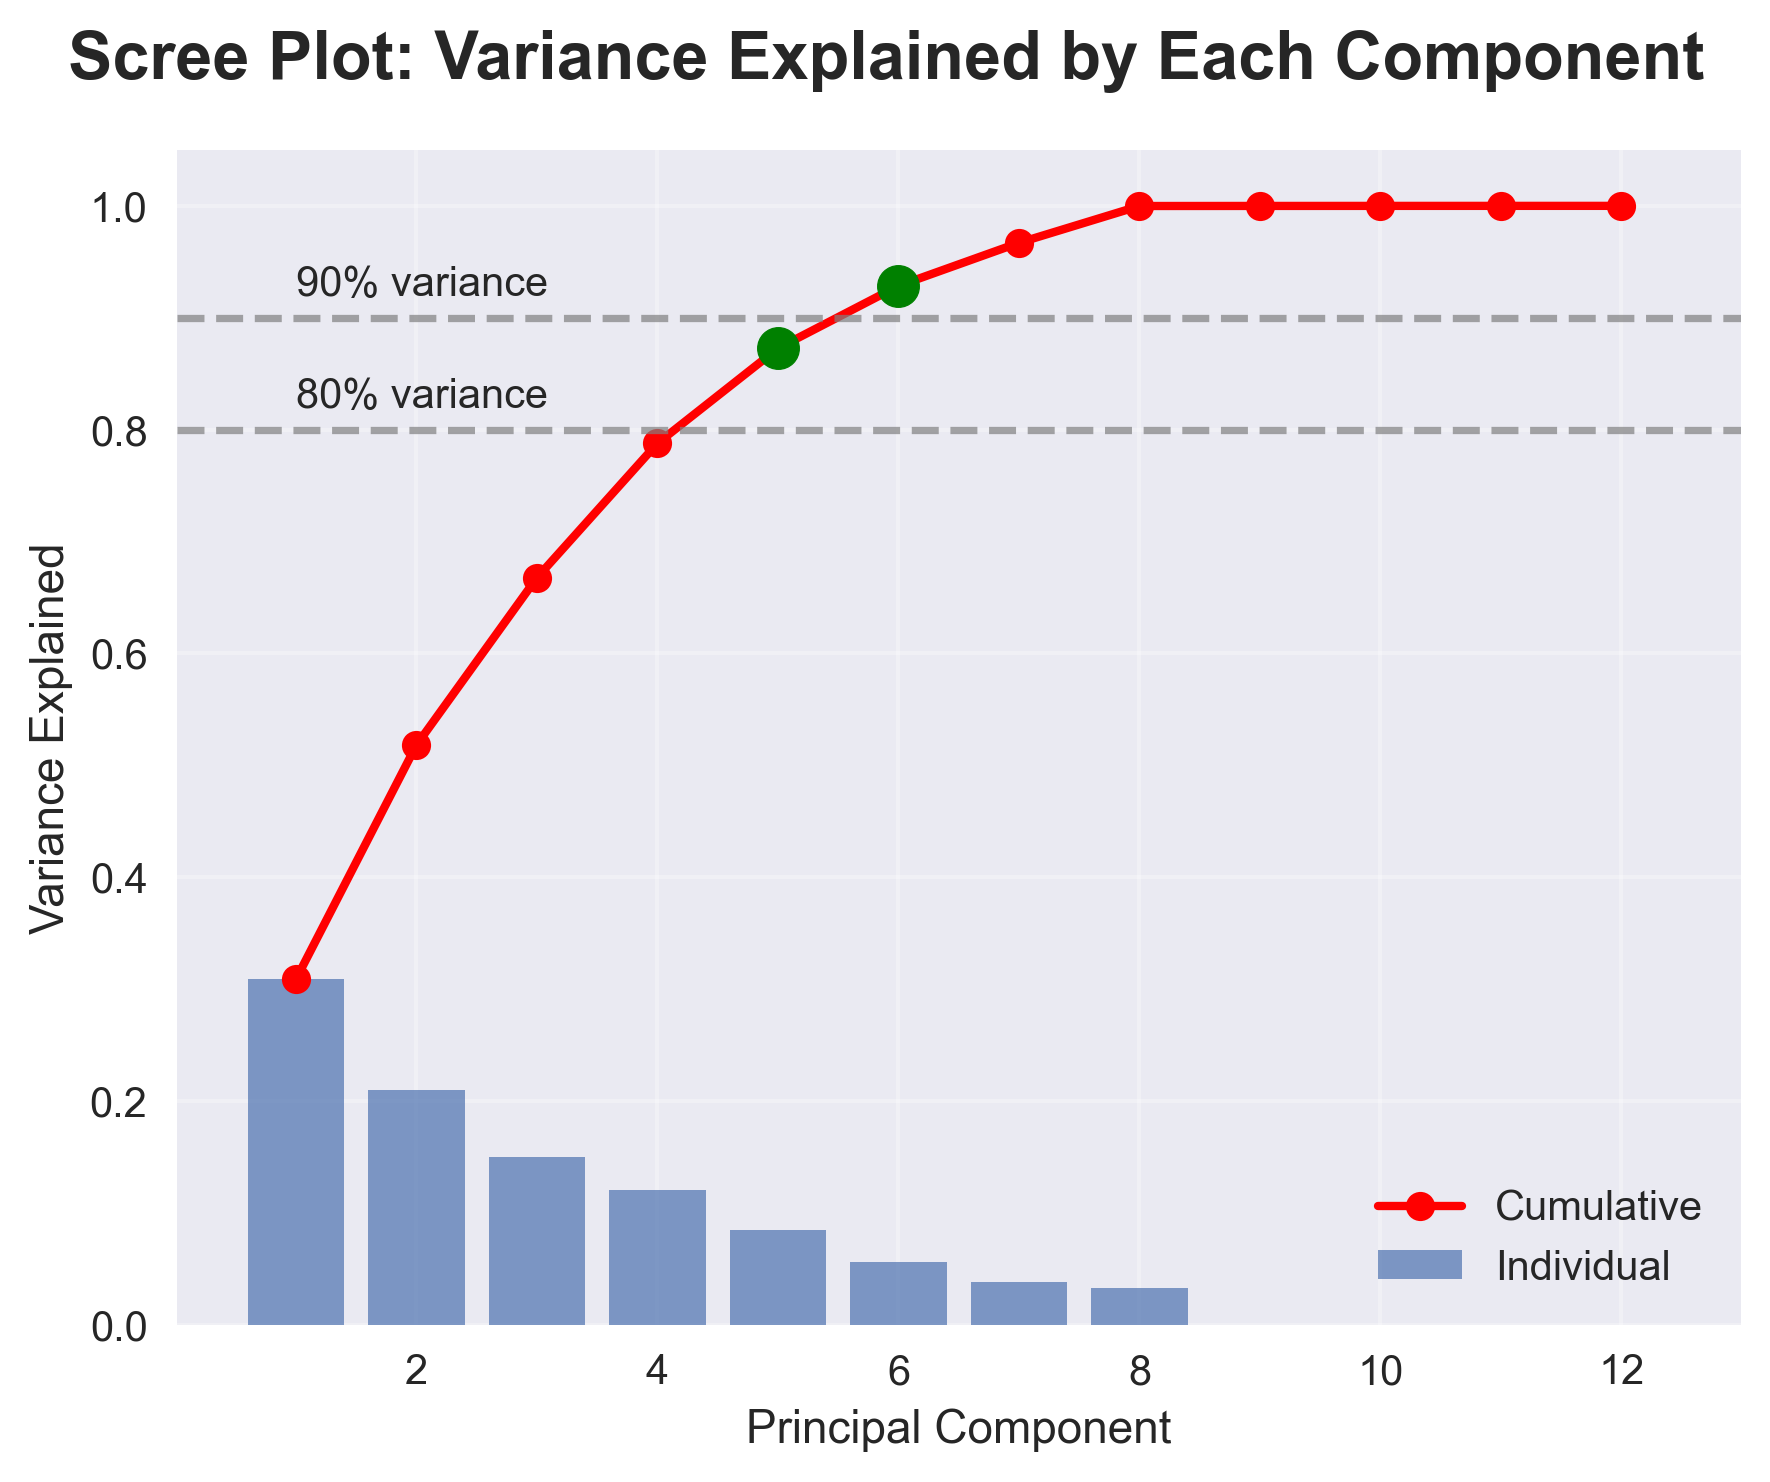
\includegraphics[width=\textwidth]{/home/msmitty/Documents/TransientBloodRheo_summerExperience/WritingMaterials/0.Figures/s2_003_screePlot.png}
    \caption{ADD CAPTION}
    \label{fig:s2003}
\end{figure}


With the first two principal components capturing over half of the physiological variation in the dataset, it is essential to understand how the original 13 blood panel variables contribute to
these components and reveals the relationships between individual donors in the transformed PC space. There are three main groups of variables that contribute to the first two principal components.
The first group includes Hematocrit (HCT), Hemoglobin (HEM), and Red Blood Cell Count (RBC), contribute significantly to PC1 in the positive direction. The second group includes Cholesterol (CHOL),
LDL Cholesterol (LDL), and Mean Corpuscular Hemoglobin Concentration (MCHC), contribute positively in the PC2 and virtually no contributions in PC1 due to the high vertical line.
Lastly the third group includes MCH, MCV, and HDL Cholesterol (HDL), which are strongly correlated with PC2 contributing negatively in PC1 and positively in PC2. The remaining variables, Fibrinogen (FIB),
Triglycerides (TRIG), and White Blood Cell Count (WBC), have weaker contributions to the principal components, indicating that they may not be as strongly associated with the overall physiological variation
captured by the first two components. (Figure \ref{fig:s2004}) There are no clear clusters in the PC space, indicating that the physiological variables do not strongly separate the donors into distinct groups based
on their blood panel results.

\begin{figure}[ht]
    \centering
    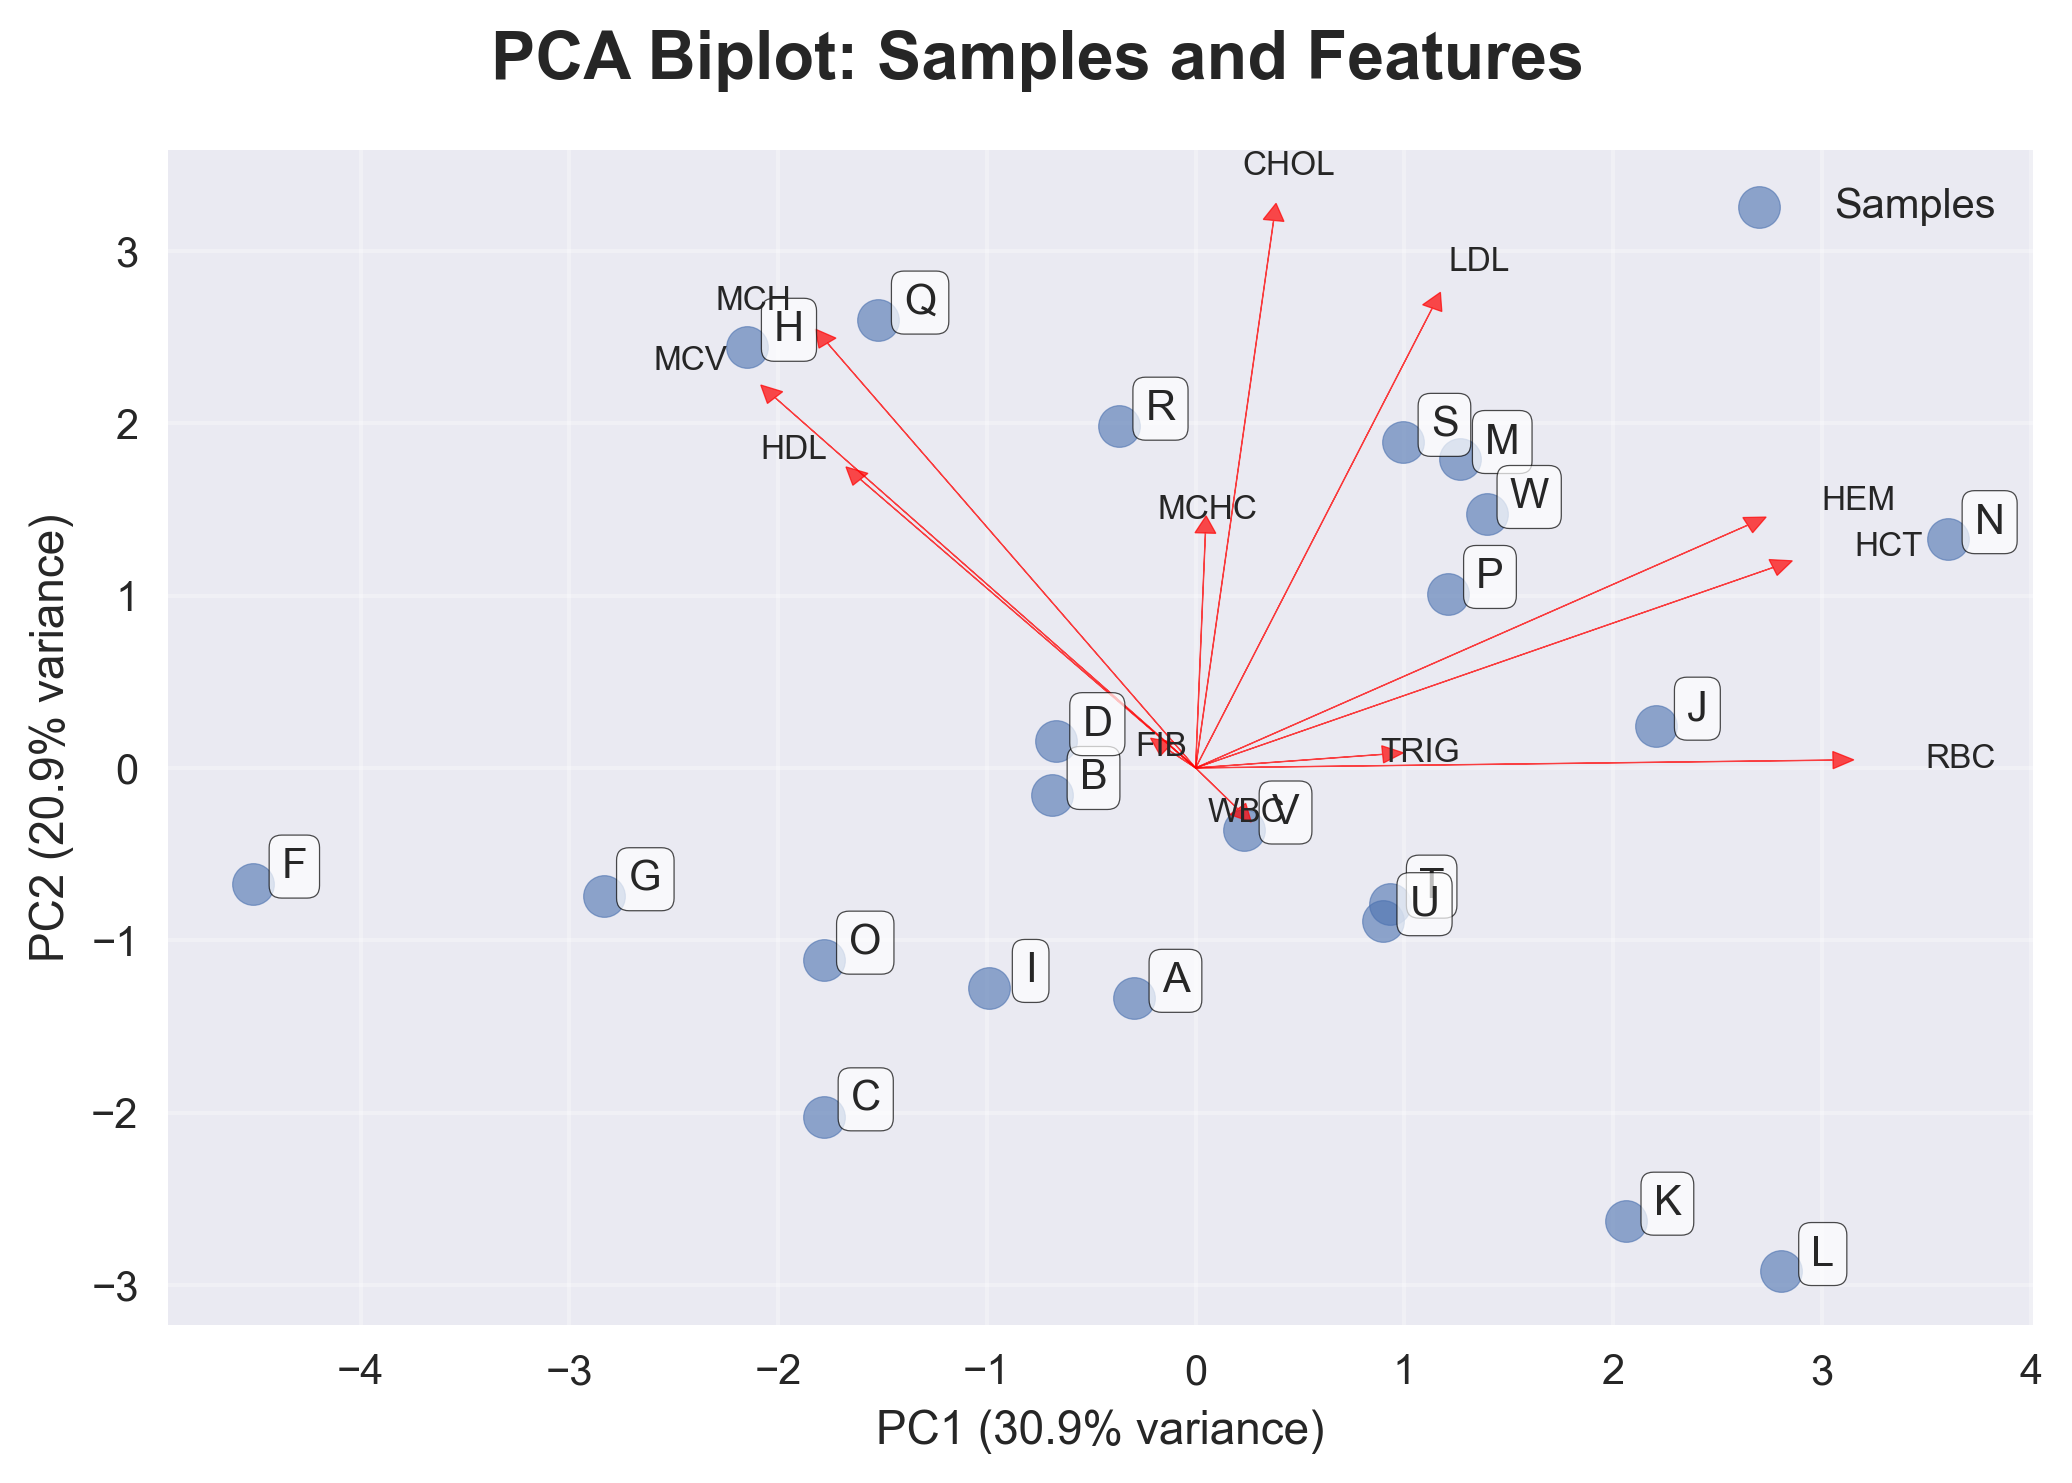
\includegraphics[width=0.5\textwidth]{/home/msmitty/Documents/TransientBloodRheo_summerExperience/WritingMaterials/0.Figures/s2_004_pcaBiplot.png}
    \caption{ADD CAPTION}
    \label{fig:s2004}
\end{figure}

The principal components' correlation to physiological parameters are described by a coefficient of a feature importance, represented by a value of $-1$ to $1$. It was found that Hematocrit (HCT),
was most correlated to PC1 and Fibrinogen (FIB) was most correlated to PC3 (figure s2005). Similar to that of the biplot, the correlations between the variables and the principal components are seen clustered into
groups. The first group includes Hematocrit (HCT), Hemoglobin (HEM), and Red Blood Cell Count (RBC), which are all positively correlated with PC1. The second group includes Cholesterol (CHOL), LDL Cholesterol (LDL),
and Mean Corpuscular Hemoglobin Concentration (MCHC), which contribute positively in the PC2.(Figure \ref{fig:s2005})

\begin{figure}[ht]
    \centering
    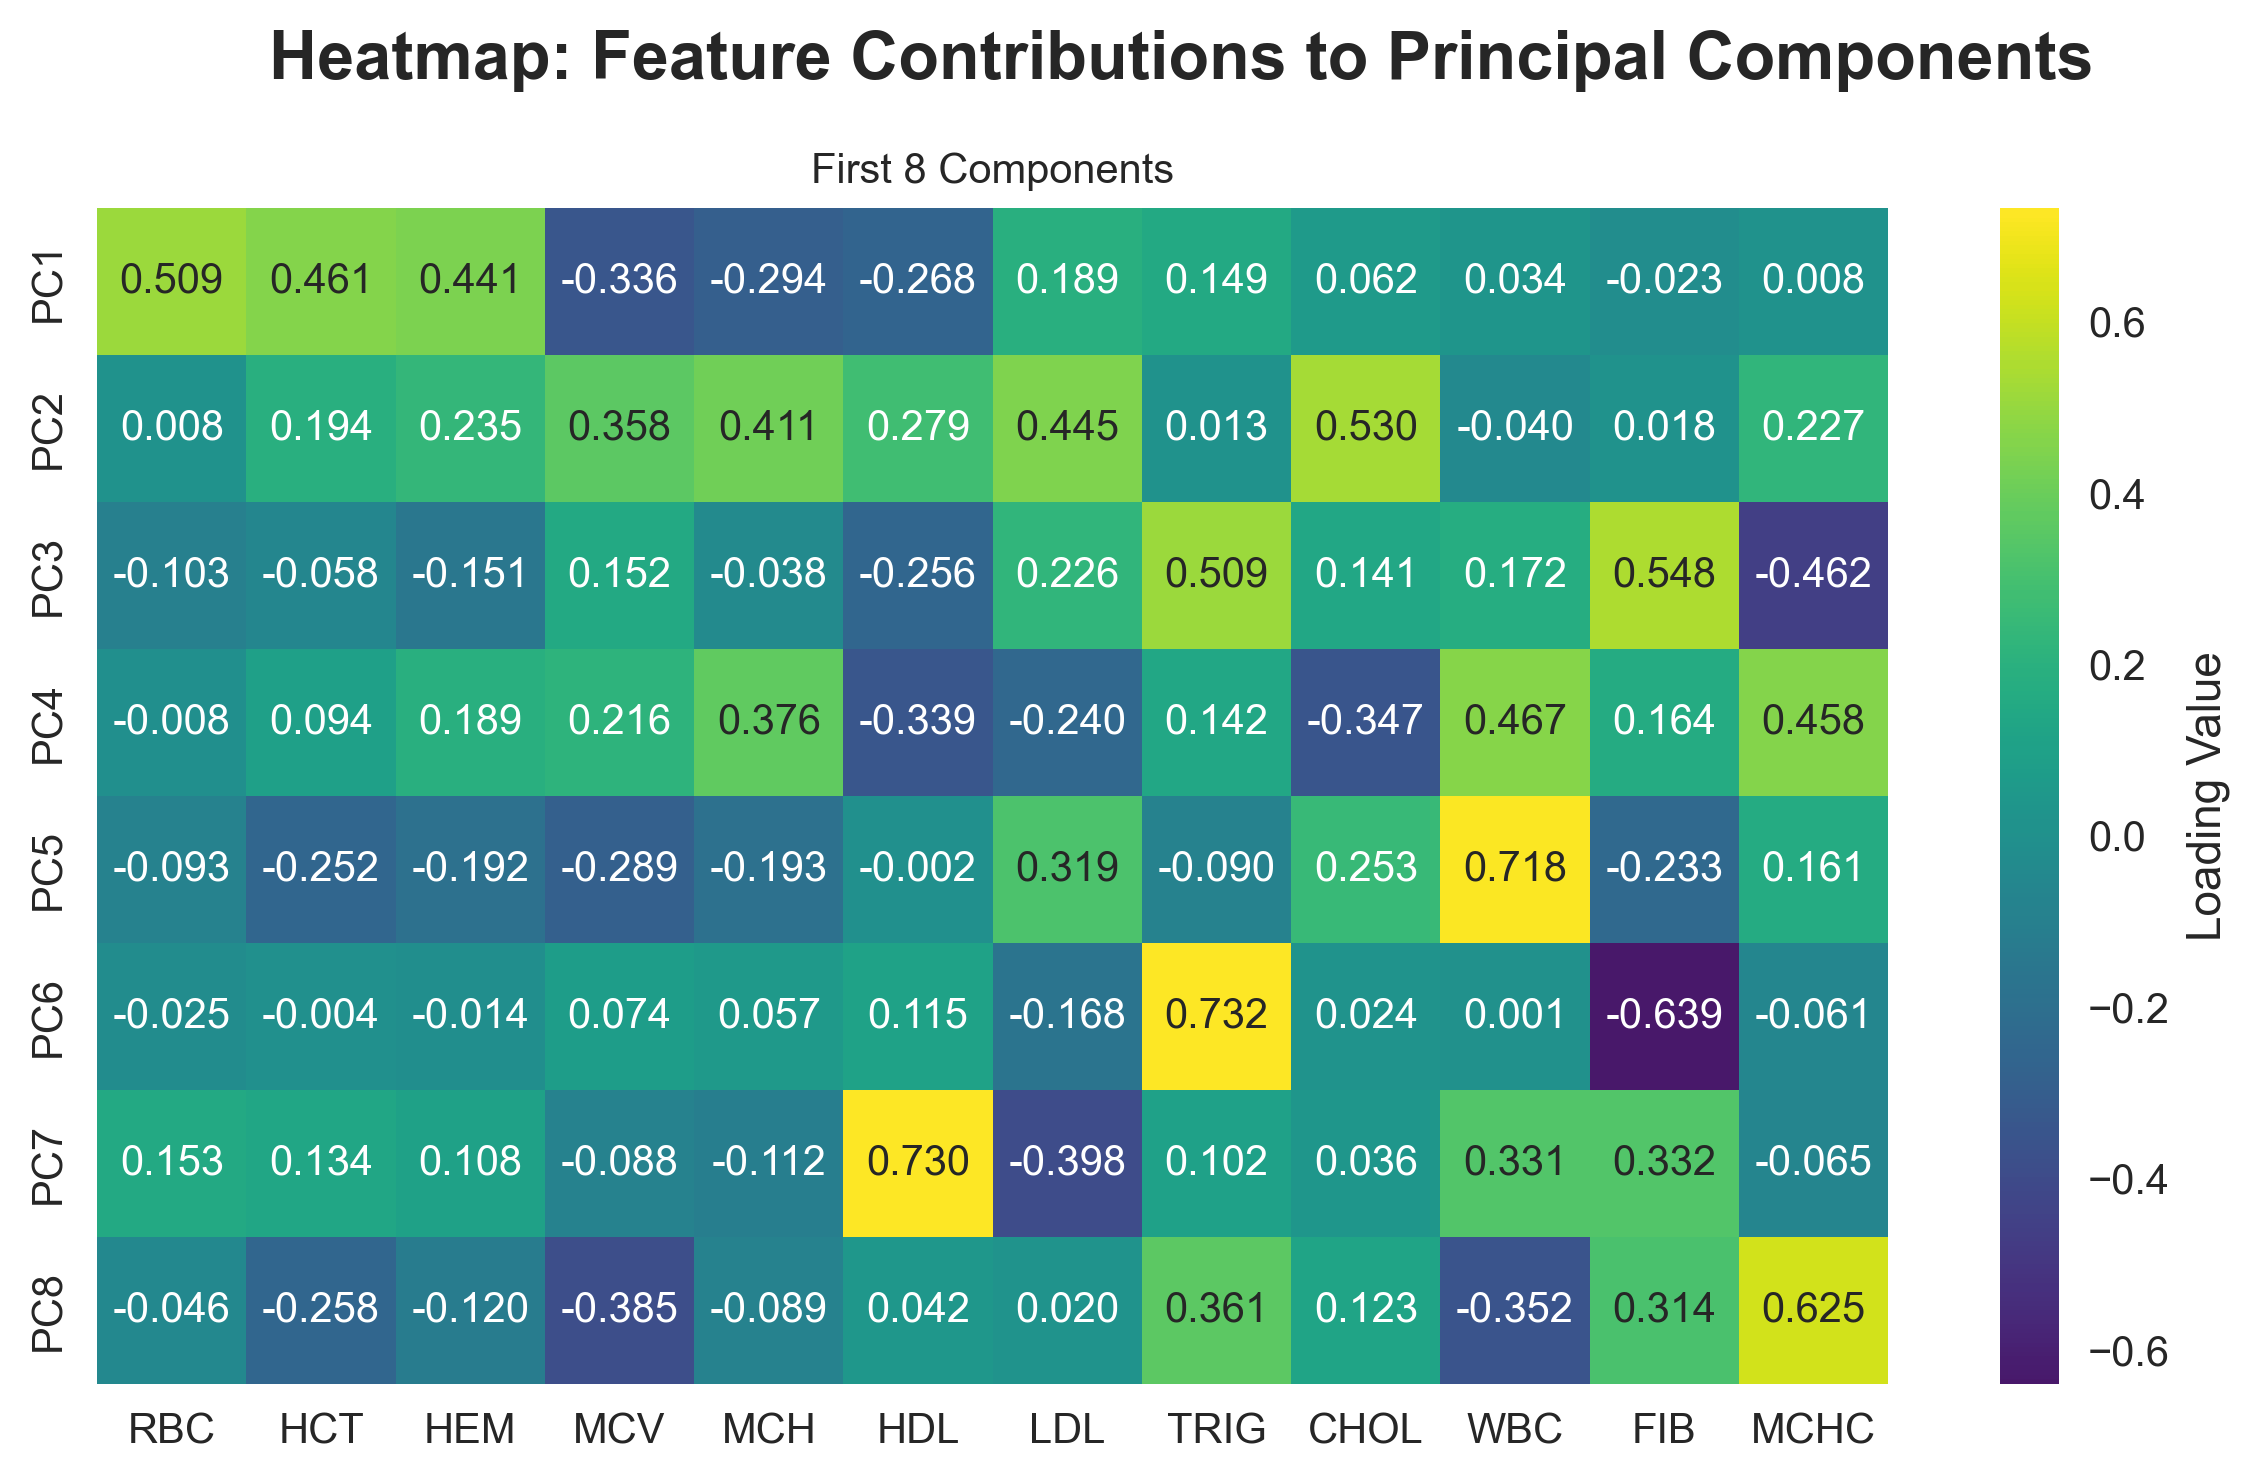
\includegraphics[width=\textwidth]{/home/msmitty/Documents/TransientBloodRheo_summerExperience/WritingMaterials/0.Figures/s2_005_pcaHeatmap.png}
    \caption{ADD CAPTION}
    \label{fig:s2005}
\end{figure}

Some basic biological interpretation of the principal components can be made based on the loadings of the physiological variables. For example, the strong loading of Hematocrit (HCT) on PC1 suggests
in conjunction with Hemoglobin (HEM) and Red Blood Cell Count (RBC) that this component captures variations in red blood cell concentration and overall blood viscosity.
Similarly, the loading of Fibrinogen (FIB) on PC3 indicates that this component may be associated with the inflammatory response and clotting dynamics in the blood. Overall, these interpretations provide
valuable insights into the underlying biological processes that drive the observed rheological behavior in the blood samples.

Utilizing the principal components as features, correlational coefficients were calculated between the principal components and the rheological parameters. The most significant correlations were found between
were between PC2 and $\mu_0$ and PC5 and $\sigma_{\gamma^O}$, with correlation coefficients of $0.478$ and $0.459$, respectively (Figure \ref{fig:s3007}). The correlation coefficients between the principal components
and the rheological parameters are generally low, indicating that the principal components do not strongly predict the rheological parameters.

\begin{figure}[ht]
    \centering
    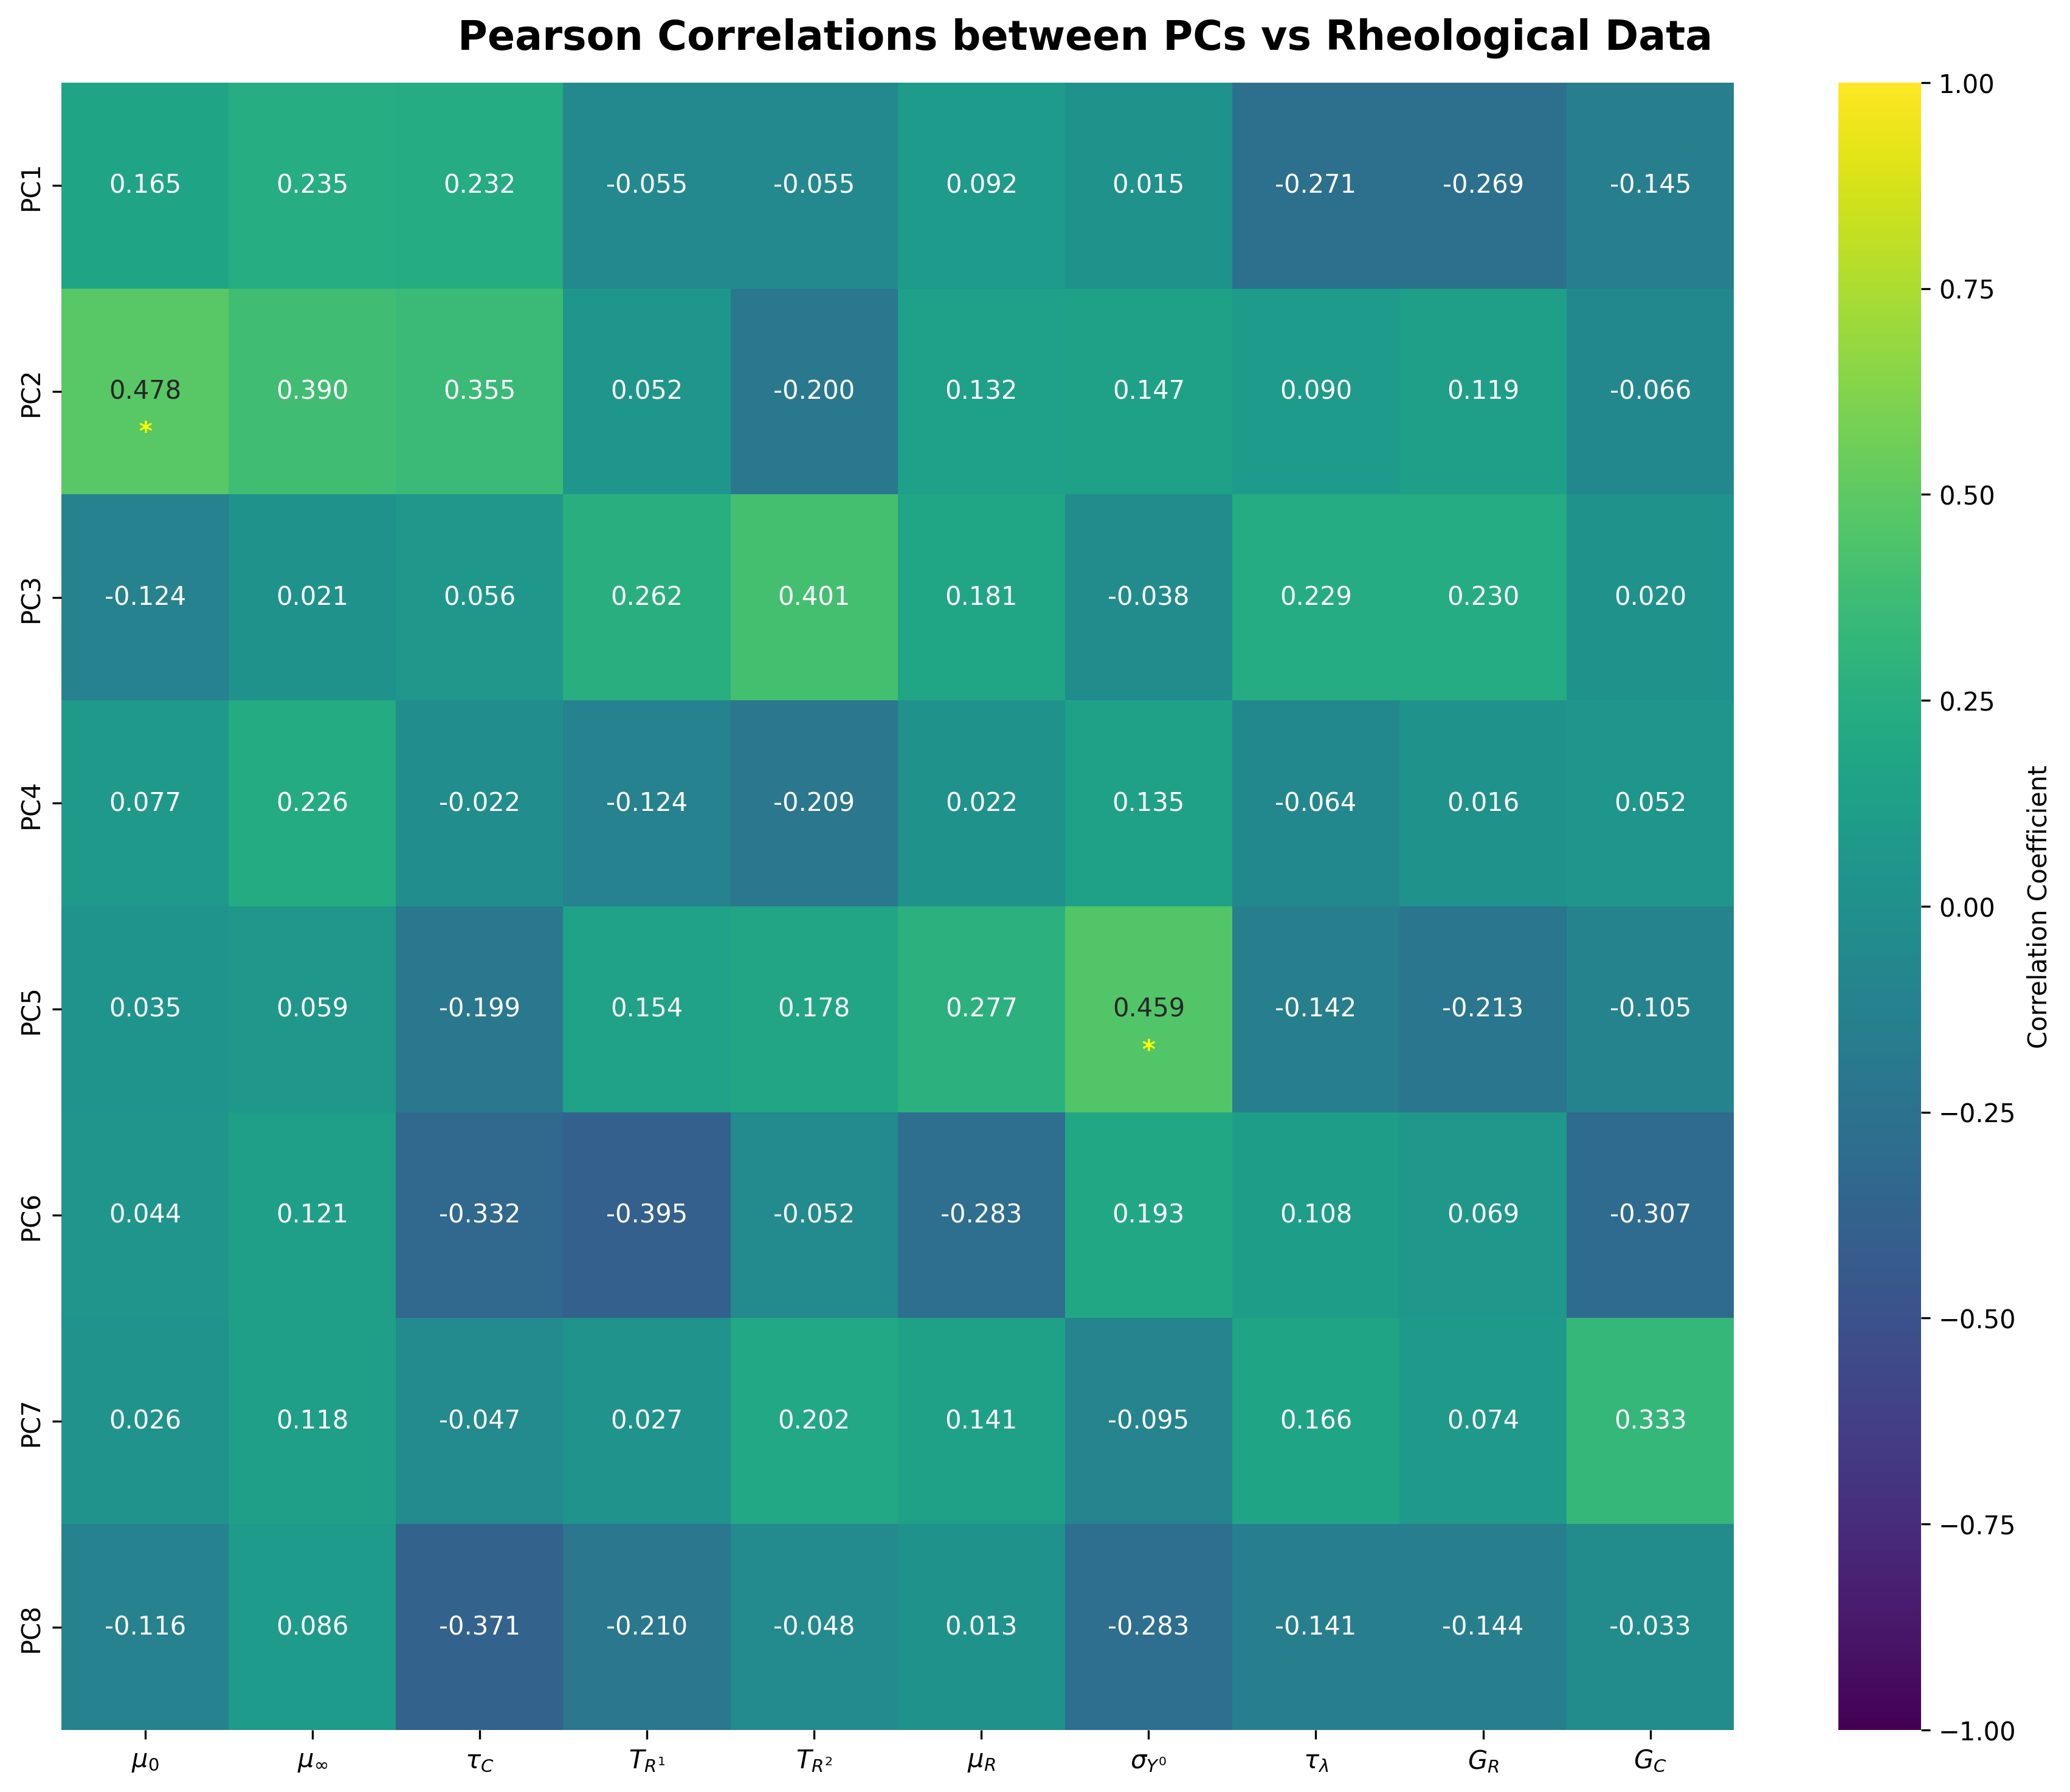
\includegraphics[width=\textwidth]{/home/msmitty/Documents/TransientBloodRheo_summerExperience/WritingMaterials/0.Figures/s3_007_corrPCAHeatmap.png}
    \caption{ADD CAPTION}
    \label{fig:s3007}
\end{figure}

One rheological parameter that was correlated to PC 2 was the zero shear viscosity ($\mu_0$), which is a measure of the viscosity of the blood at low shear rates. To understand this correlation between the data was plotted to show
this correlation (Figure \ref{fig:pc2-mu}). There is an outlier for observation S. 15 observations were within the 95\% confidence interval. The correlation coefficient of $r=0.478$ suggests that there is moderate positive correlation between these values.
With $\mu_0$ showing a correlation with PC2 that means that physiological parameters correlated to PC2 may also be correlated to $\mu_0$. The correlation between the physiological variables and $\mu_0$ were plotted show
consistency in the results, as what would be expected (figure ). The individual variables have a low positive correlation with $\mu_0$ (figure ), but when combined the results resemble that of the plot with PC2 vs $\mu_0$.

\begin{figure}[ht]
    \centering
    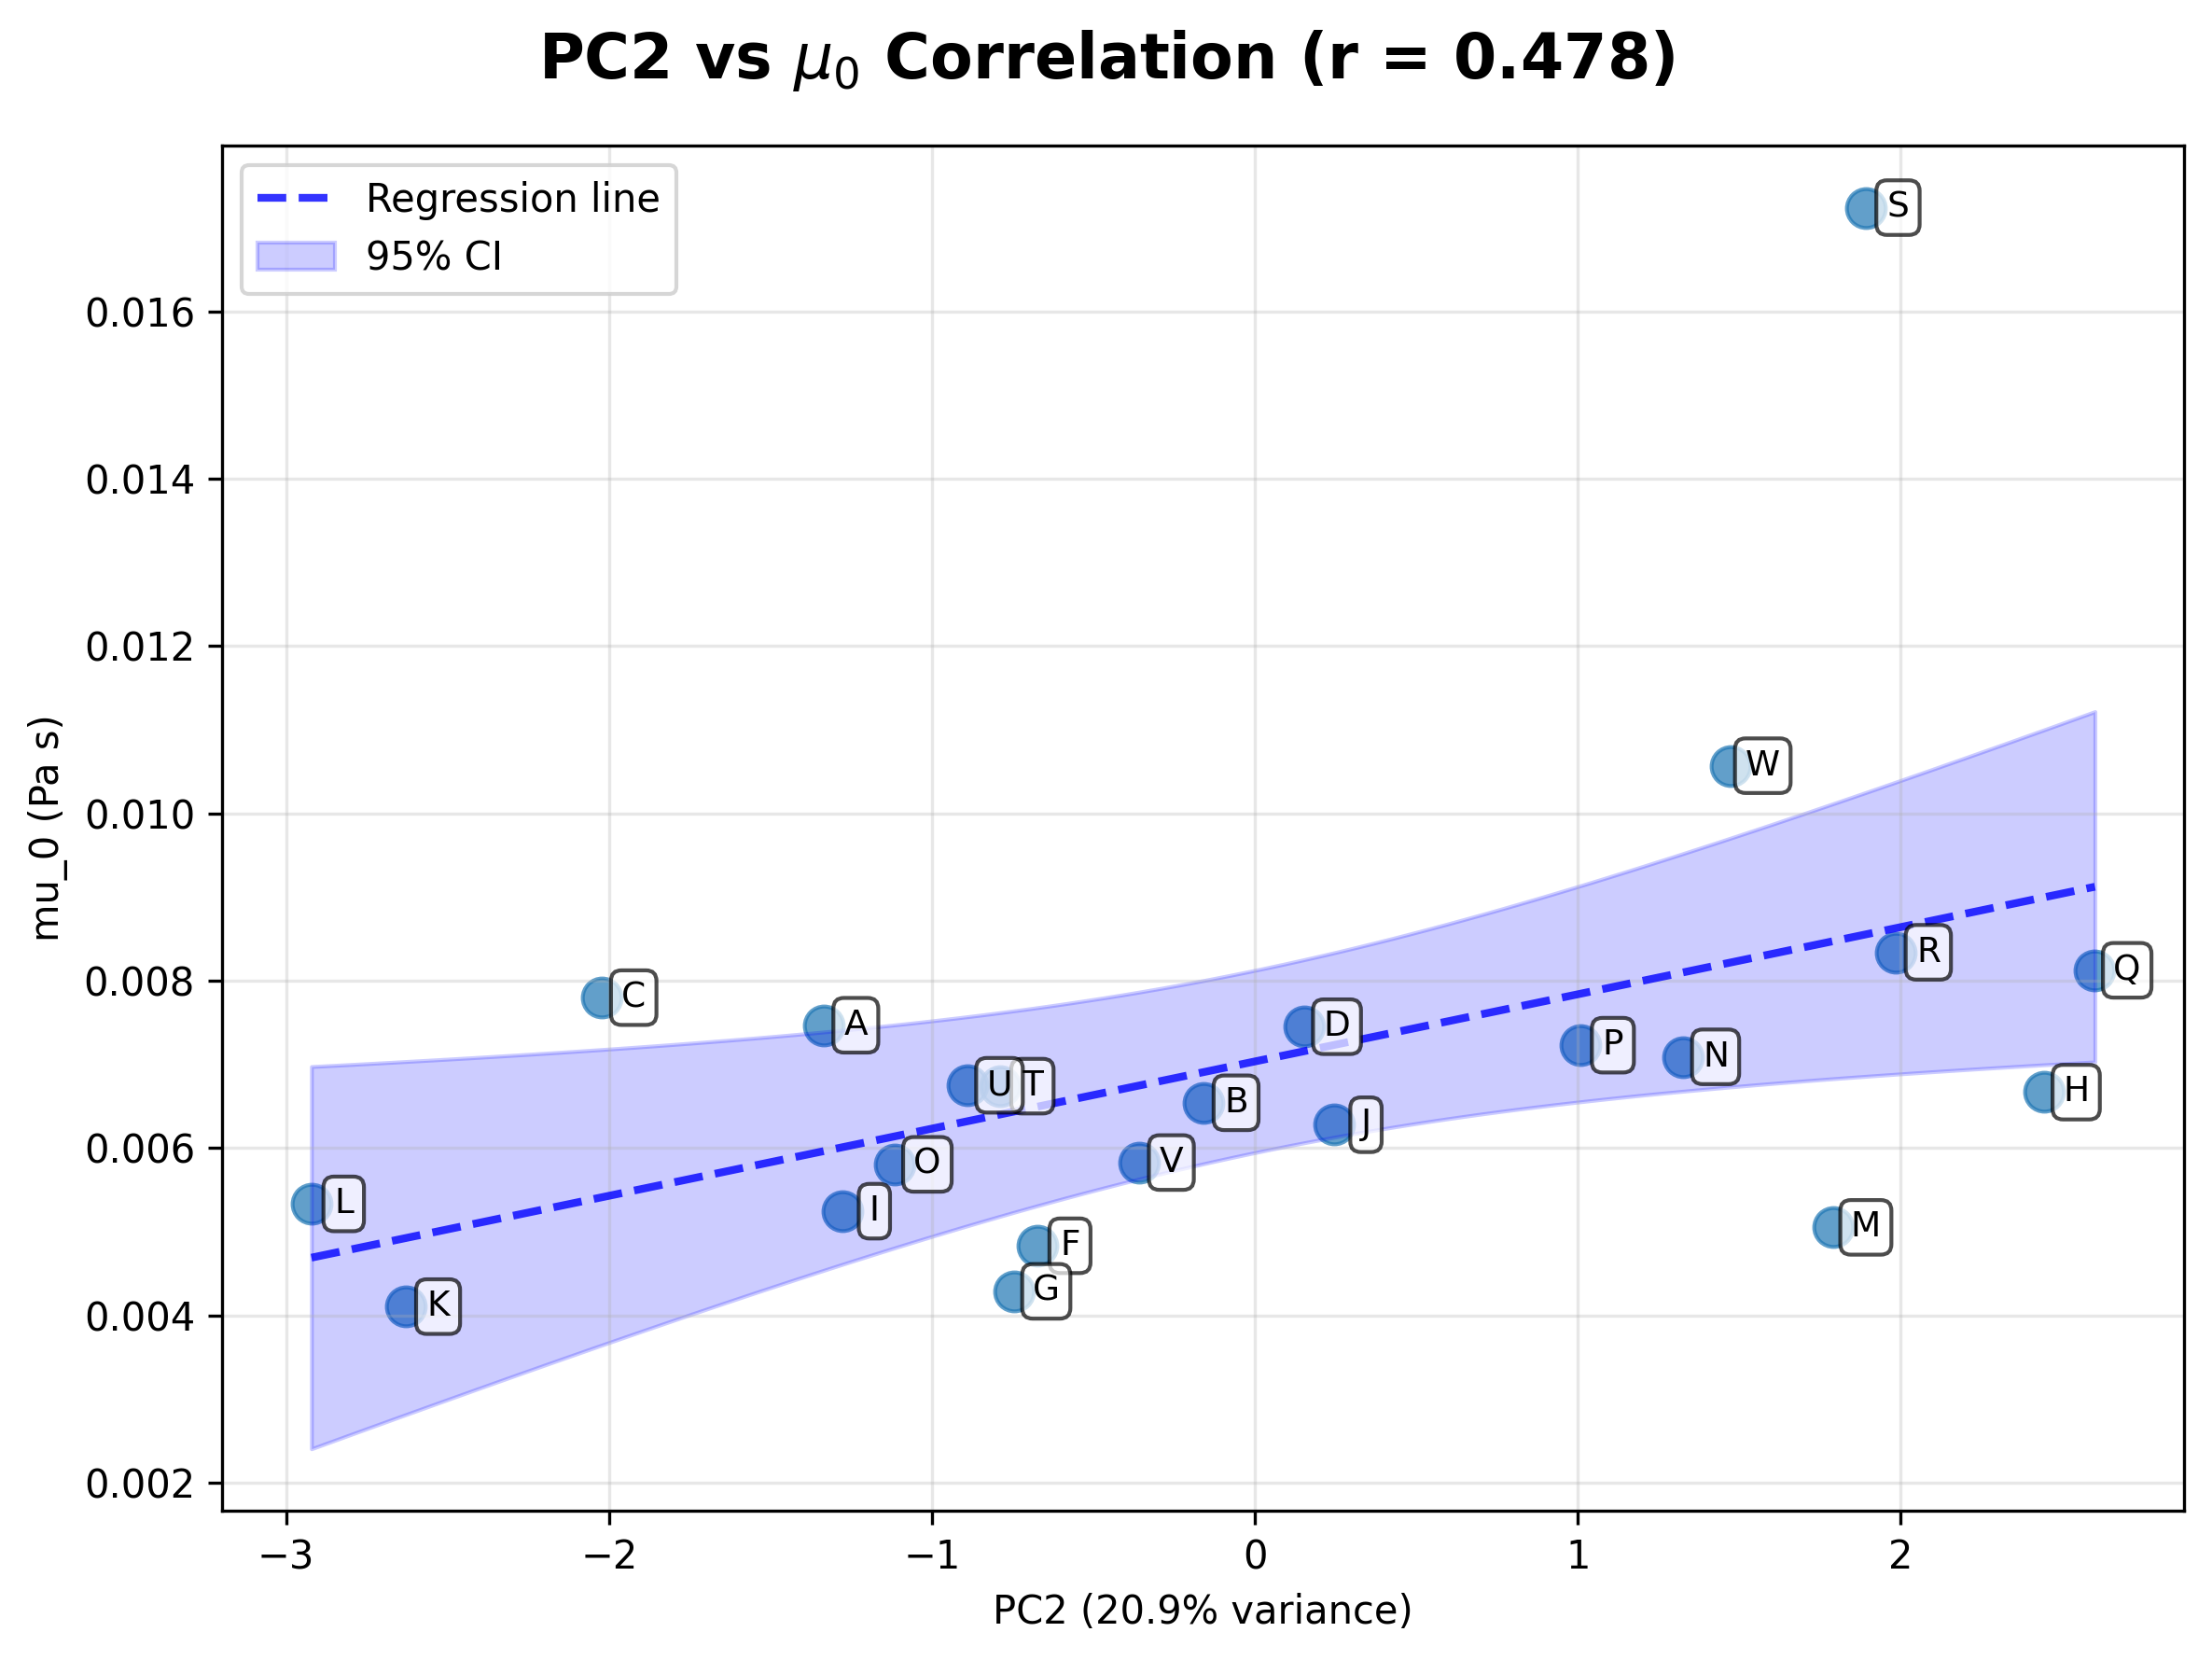
\includegraphics[width=\textwidth]{/home/msmitty/Documents/TransientBloodRheo_summerExperience/WritingMaterials/0.Figures/pc2_mu_0 (Pa s)_correlation.png}
    \caption{ADD CAPTION}
    \label{fig:pc2-mu}
\end{figure}

The results from the k-fold cross validation signified limited strength in the validity of the Gaussian Process Regression model (Figure \ref{fig:s4011}). The $R^2_{CV}$ metric resulted in negative values indicating that the model performs worse
than simply predicting the mean. There is no strength of evidence to suggest a connection between the physiological parameters and the rheological parameters; moreover, the converse can not be assumed that there is not a connection.
Further investigation in specific variables may have more influence than the selected.

\begin{figure}[ht]
    \centering
    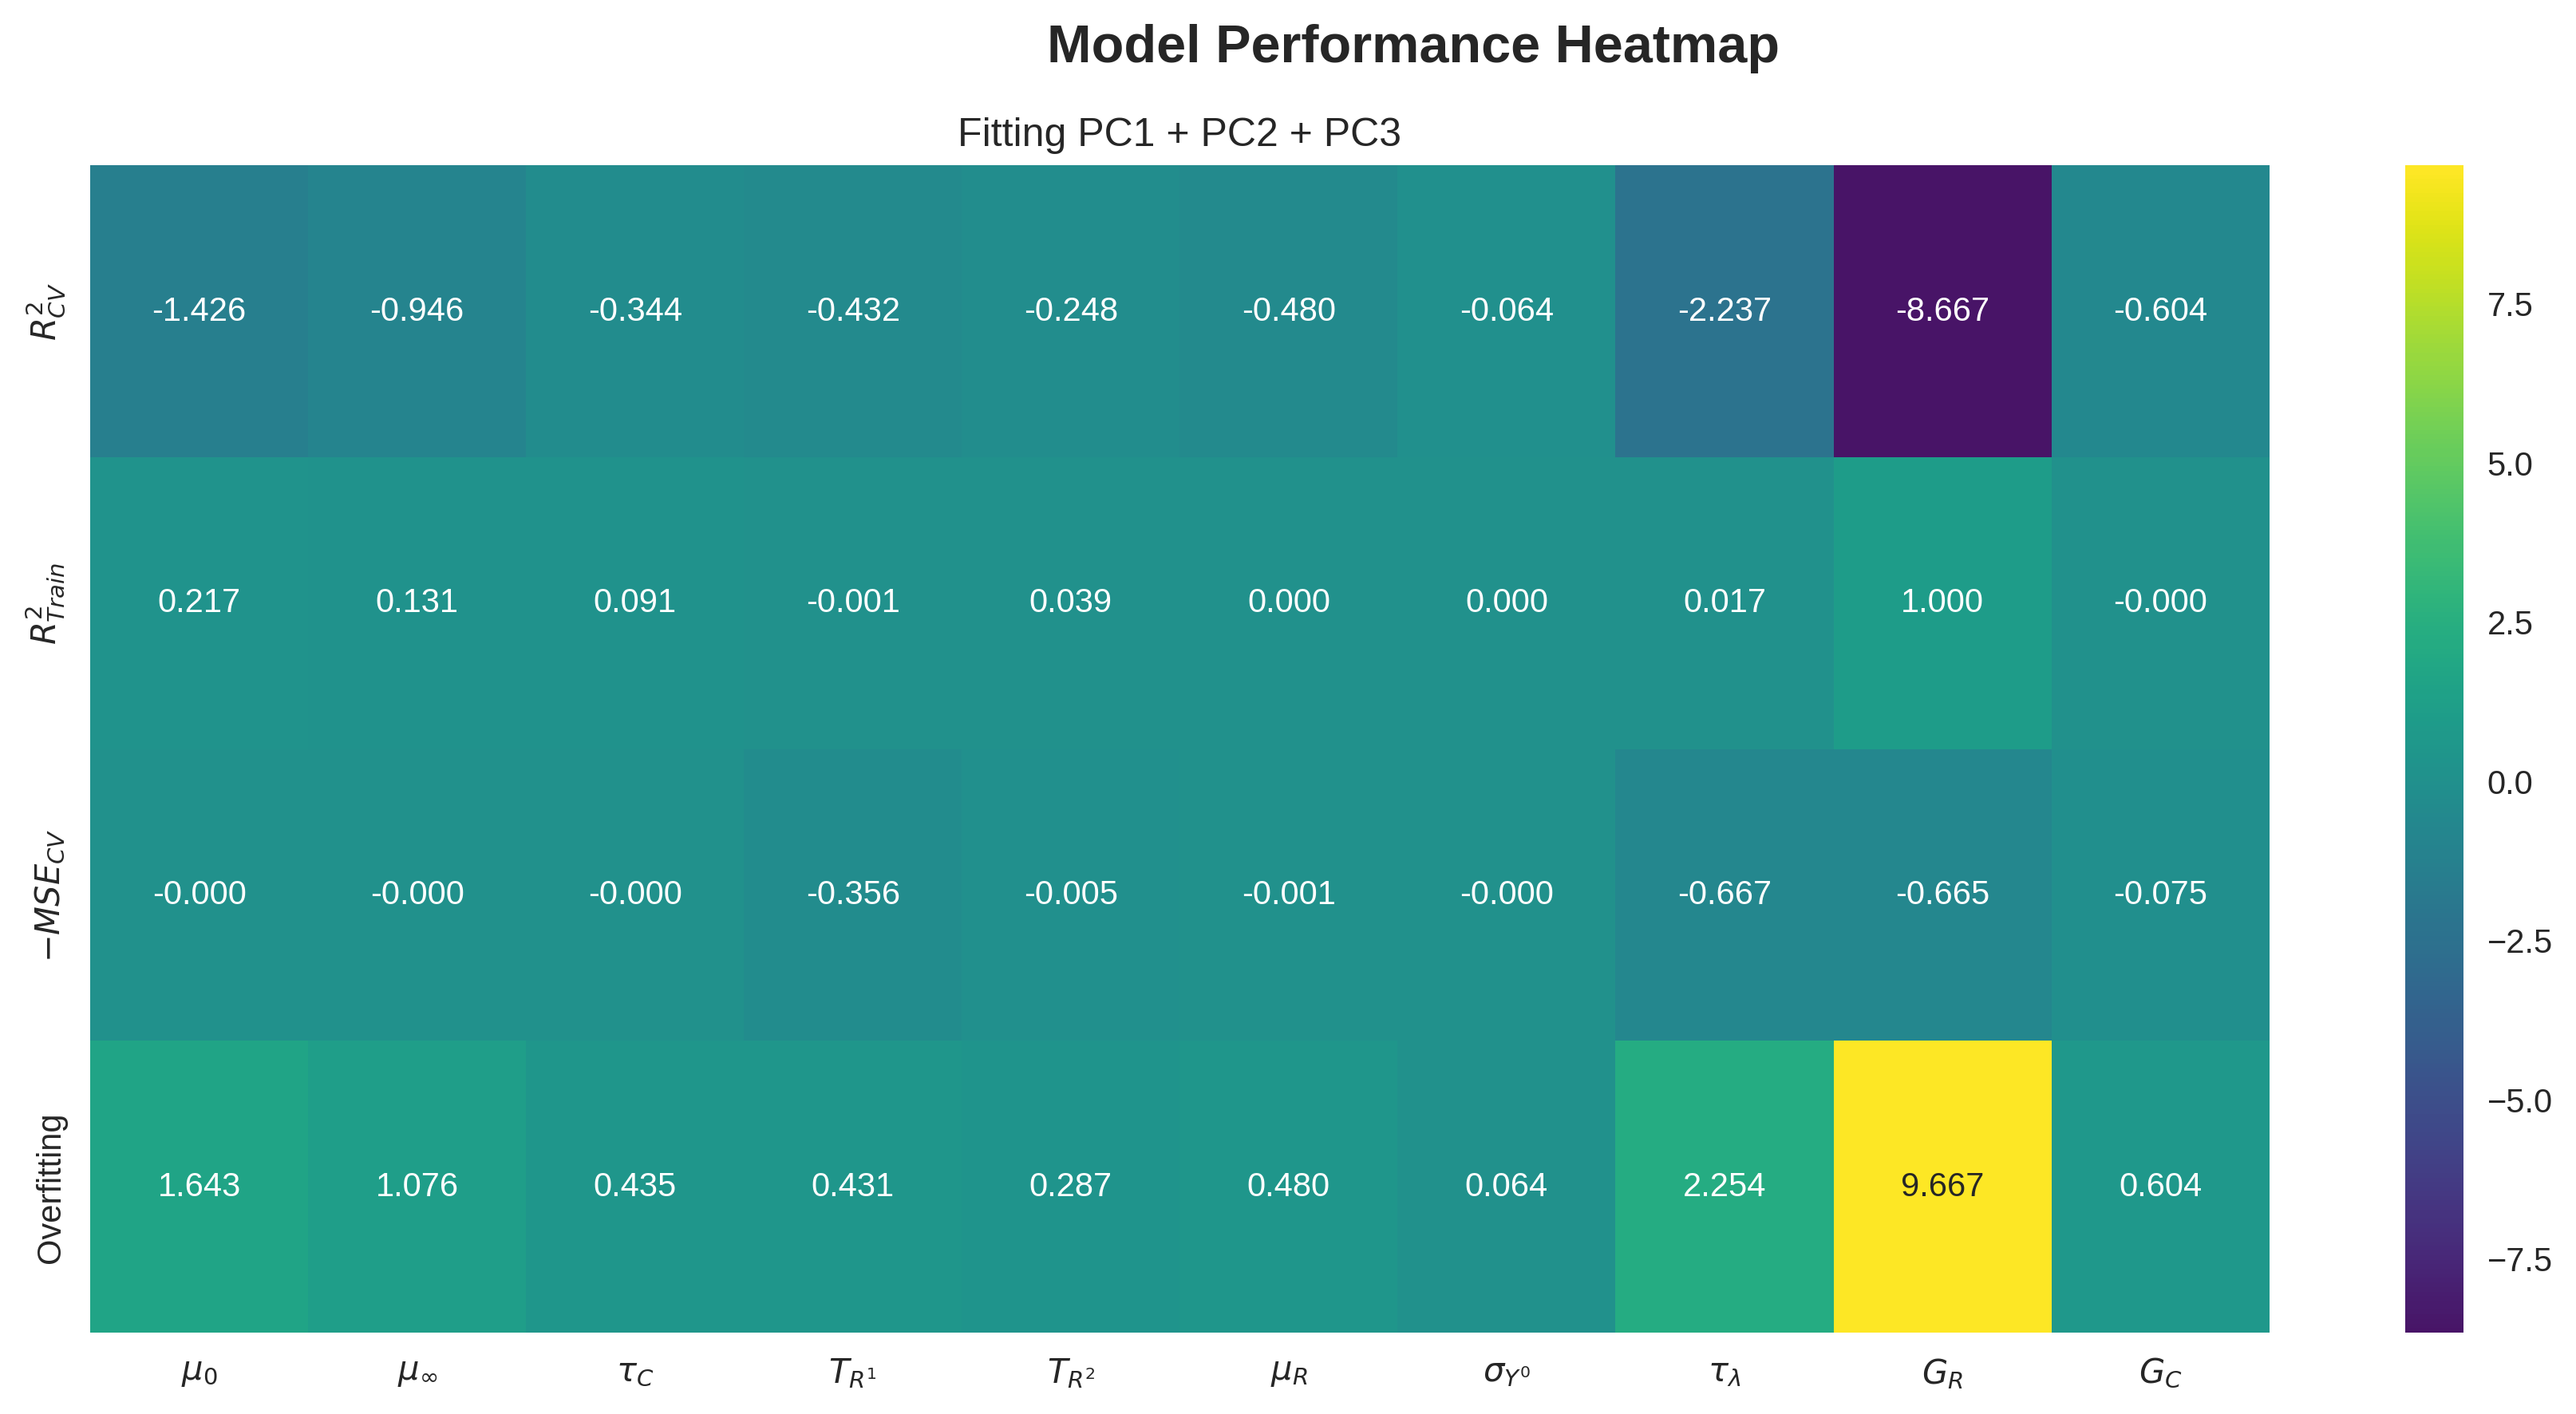
\includegraphics[width=\textwidth]{/home/msmitty/Documents/TransientBloodRheo_summerExperience/WritingMaterials/0.Figures/s4_011_gprPerformanceHeatmap.png}
    \caption{ADD CAPTION}
    \label{fig:s4011}
\end{figure}


Synthetic data generation was employed as a critical strategy to address the fundamental challenge posed by the limited sample size ($n=22$)
relative to the high-dimensional feature space in this study. 

The analysis identifies $n\approx 75$ as a critical threshold where diminishing returns in model performance become apparent (Figure \ref{fig:s5012}).
Beyond this sample size, most well-performing parameters show only marginal improvements, indicating that the models have effectively
learned the underlying relationships between physiological variables and rheological behavior. This finding provides crucial guidance for
future experimental design, suggesting that studies requiring similar predictive accuracy should target sample sizes in the $75-100$ range.

\begin{figure}[ht]
    \centering
    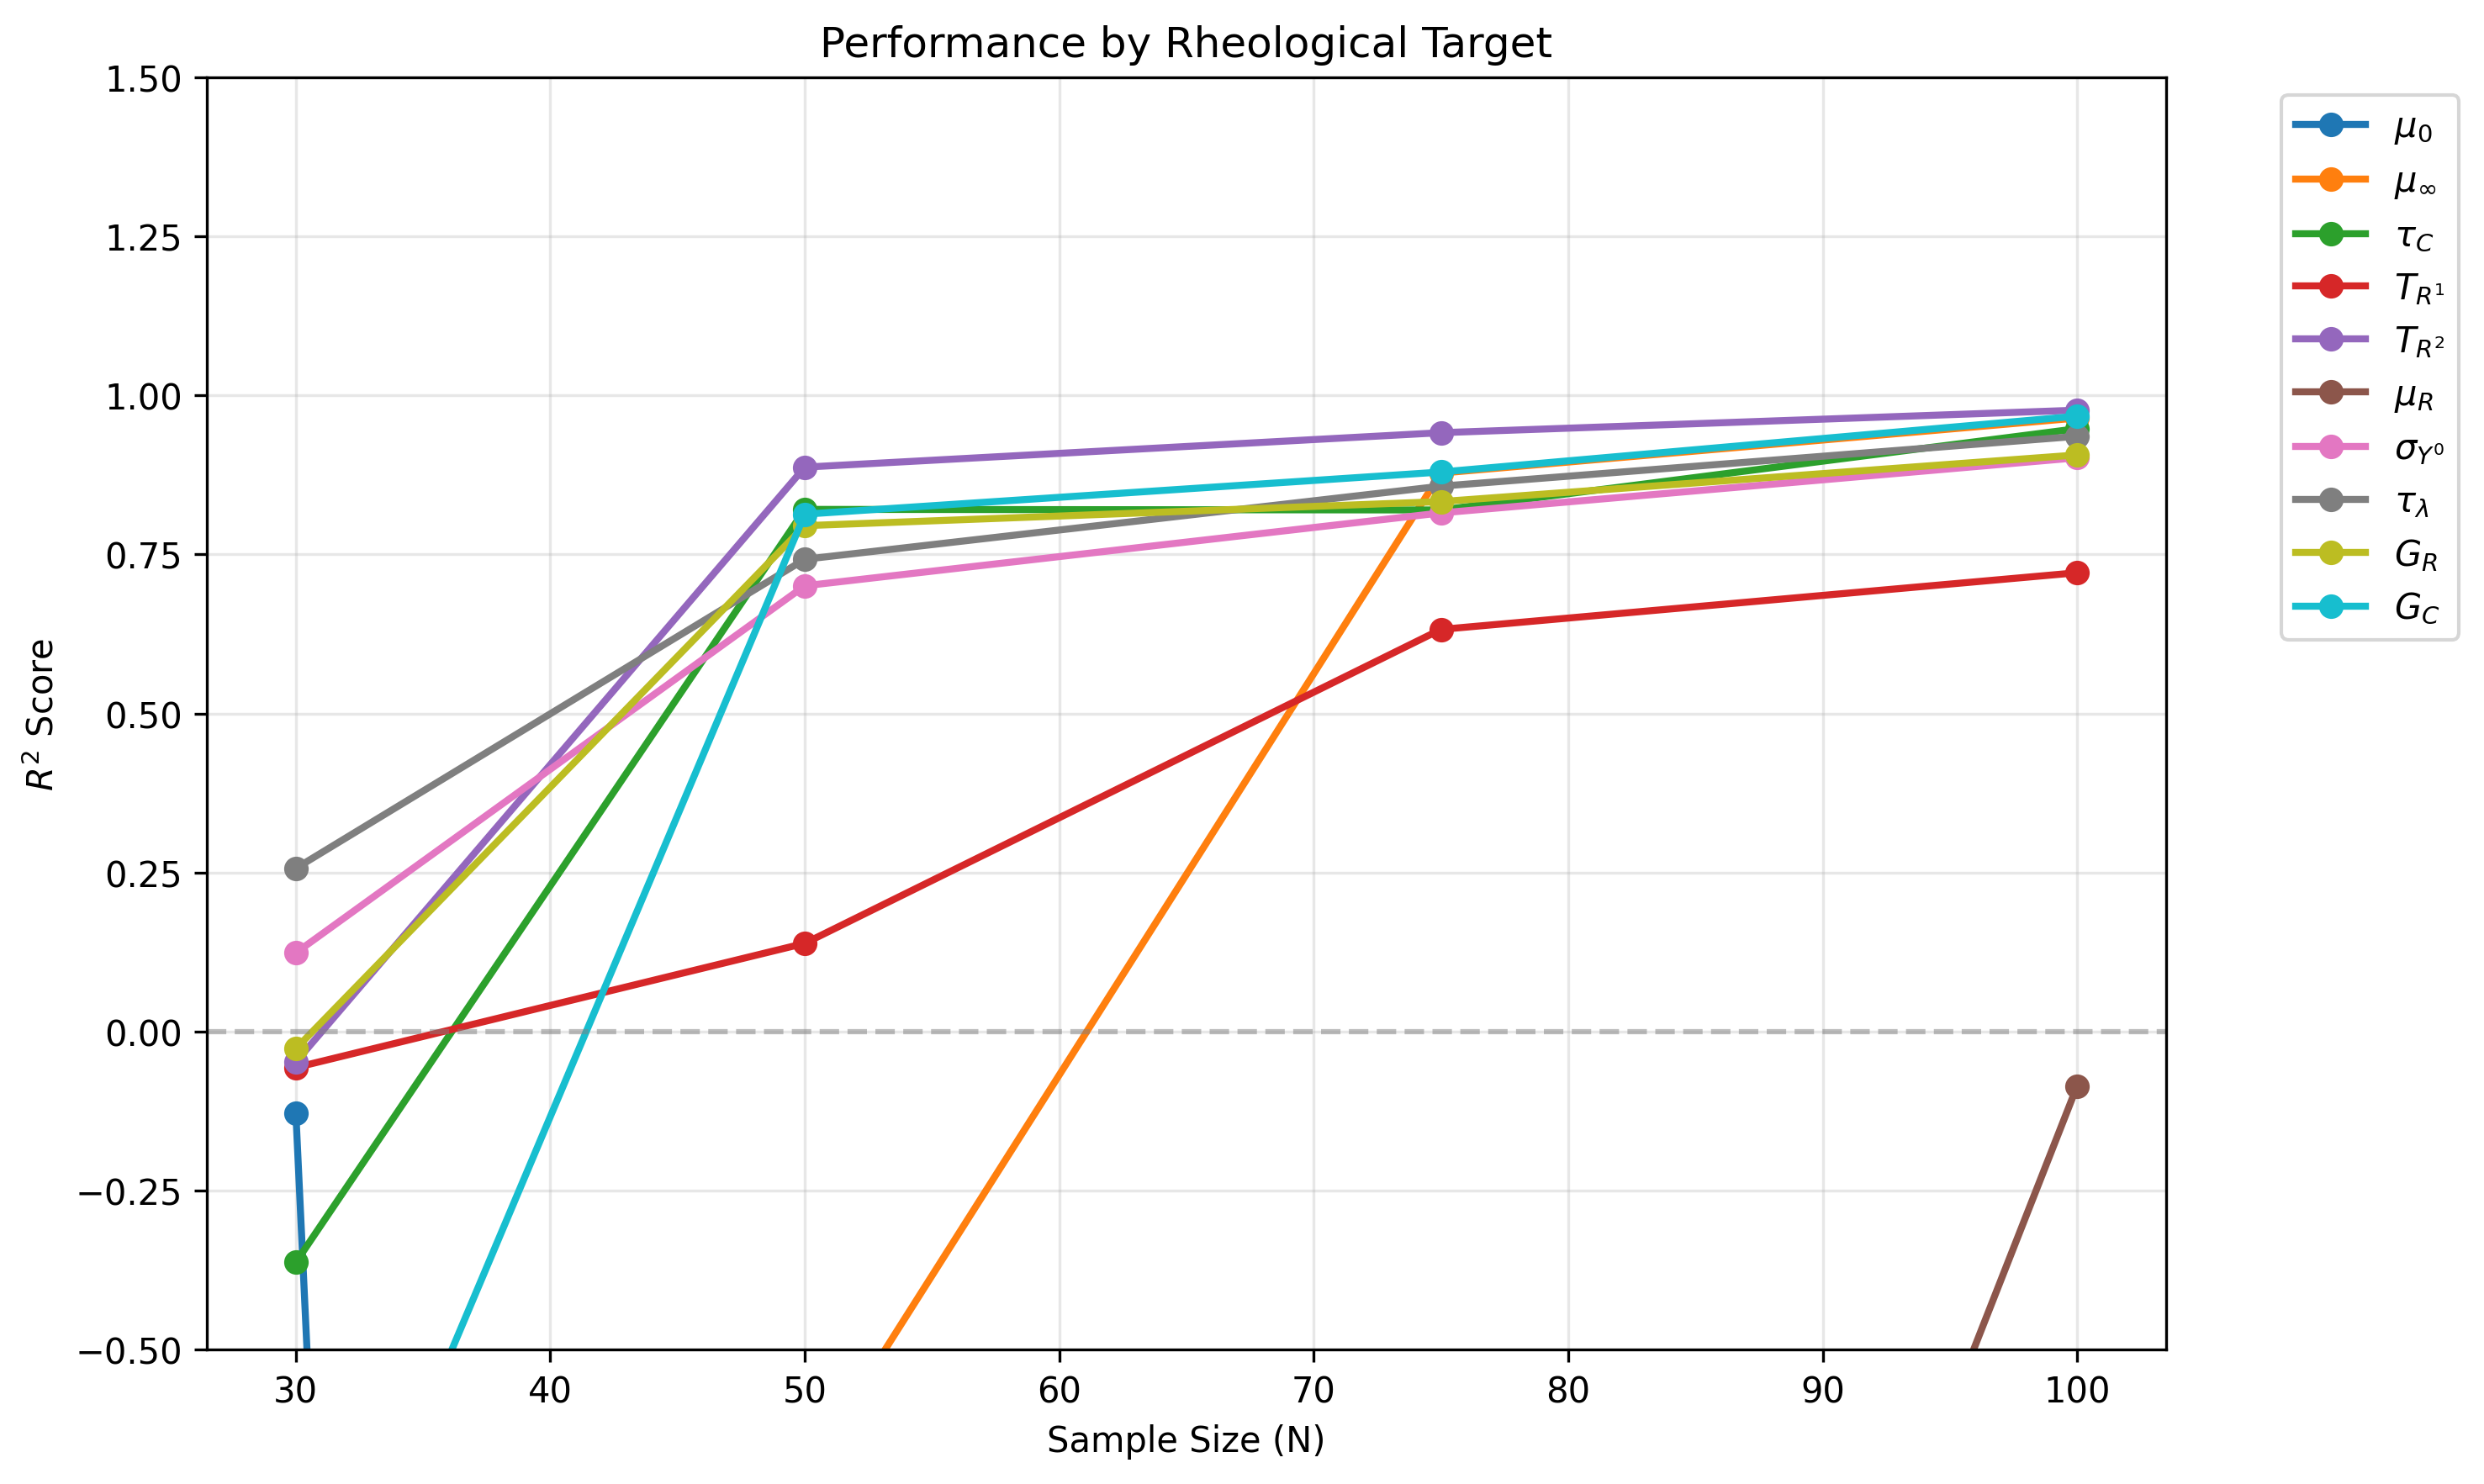
\includegraphics[width=\textwidth]{/home/msmitty/Documents/TransientBloodRheo_summerExperience/WritingMaterials/0.Figures/s5_012_knnSynthetic.png}
    \caption{Cross-validation performance ($R^2$) of machine learning models predicting rheological parameters as a function of
    synthetic dataset size. Each line represents a different rheological parameter from the constitutive model.
    Eight parameters show strong convergence to $R^2 > 0.85$ by n=75, while two parameters ($\mu_0 and \mu_R$) demonstrate persistent
    poor performance across all sample sizes, suggesting fundamental challenges in their prediction from standard physiological variables.}
    \label{fig:s5012}
\end{figure}

Some of the predicted values never reached a positive $R^2_{CV}$ value (Figure \ref{tab:noSyn}). While the majority of parameters can be successfully
predicted from physiological data once adequate sample sizes are achieved,
the two problematic parameters may require alternative measurement approaches or the inclusion of additional biomarkers not typically
assessed in standard blood panels. Future studies should consider incorporating more specialized measurements, such as detailed protein
profiling or cellular morphology assessments, to improve prediction of these challenging rheological parameters.

\begin{table}[ht]
    \centering
    \caption{Rheological Parameter that never reached a positive $R^2_{CV}$}
    \begin{tabular}{l}
        Rheological Parameter\\
        \hline
        $\mu_0$\\
        $\mu_R$
    \end{tabular}
    \label{tab:noSyn}
\end{table}












% Discussion
\newpage
\section{Discussion}
Discussion section here.



% Future Directions
\newpage
\section{Future Directions}
Future directions section here.

% Conclusion
\newpage
\section{Conclusion}
Conclusion section here.

% Acknowledgments
\newpage
\section{Acknowledgments}

- Sean Farrington
- Norman J. Wagner

% Resources
\newpage
\section{Resources}
Resources section here.

% Accronyms
\newpage
\section{Acronyms}
\begin{itemize}
    \item GPR: Gaussian Process Regression
    \item PC: Principal Component
    \item ML: Machine Learning
    \item PCA: Principal Component Analysis
    \item CV: Cross-Validation
    \item KFCV: K-Fold Cross-Validation
    \item MSE: Mean Squared Error
    \item RMSE: Root Mean Squared Error
    \item MAE: Mean Absolute Error
    \item $R^2$: Coefficient of Determination
    \item CI: Confidence Interval
    \item PCs: Principal Components
\end{itemize}

% References
\newpage
%\printbibliography[title=References]

% Appendices (if needed)
\newpage
\appendix

\section{Supplementary Data}
\label{app:supplementary}

[Include supplementary figures, tables, or data here]

\end{document}
